% !TEX program = xelatex
\documentclass[a4paper,14pt,oneside,openany]{memoir}

%%% Задаем поля, отступы и межстрочный интервал %%%
\usepackage{amsmath}
\usepackage[left=30mm, right=15mm, top=20mm, bottom=20mm]{geometry} % Пакет geometry с аргументами для определения полей
\pagestyle{plain} % Убираем стандарные для данного класса верхние колонтитулы с заголовком текущей главы, оставляем только номер страницы снизу по центру
\parindent=1.25cm % Абзацный отступ 1.25 см, приблизительно равно пяти знакам, как по ГОСТ
\usepackage{indentfirst} % Добавляем отступ к первому абзацу
%\linespread{1.3} % Межстрочный интервал (наиболее близко к вордовскому полуторному) - тут вместо этого используется команда OnehalfSpacing*

%%% Задаем языковые параметры и шрифт %%%

\usepackage[english, russian]{babel}                % Настройки для русского языка как основного в тексте
\babelfont{rm}{Times New Roman}                     % TMR в качестве базового roman-щрифта

%%% Задаем стиль заголовков и подзаголовков в тексте %%%

\setsecnumdepth{subsection} % Номера разделов считать до третьего уровня включительно, т.е. нумеруются только главы, секции, подсекции
\renewcommand*\chapterheadstart{} % Переопределяем команду, задающую отступ над заголовком, чтобы отступа не было
\renewcommand*\printchaptername{} % Переопределяем команду, печатающую слово "Глава", чтобы оно не печалось
%\renewcommand*\printchapternum{} % То же самое для номера главы - тут не надо, номер главы оставляем
\renewcommand*\chapnumfont{\normalfont\bfseries} % Меняем стиль шрифта для номера главы: нормальный размер, полужирный
\renewcommand*\afterchapternum{\hspace{1em}} % Меняем разделитель между номером главы и названием
\renewcommand*\printchaptertitle{\normalfont\bfseries\centering\MakeUppercase} % Меняем стиль написания для заголовка главы: нормальный размер, полужирный, центрированный, заглавными буквами
\setbeforesecskip{20pt} % Задаем отступ перед заголовком секции
\setaftersecskip{20pt} % Ставим такой же отступ после заголовка секции
\setsecheadstyle{\raggedright\normalfont\bfseries} % Меняем стиль написания для заголовка секции: выравнивание по правому краю без переносов, нормальный размер, полужирный
\setbeforesubsecskip{20pt} % Задаем отступ перед заголовком подсекции
\setaftersubsecskip{20pt} % Ставим такой же отступ после заголовка подсекции
\setsubsecheadstyle{\raggedright\normalfont\bfseries}  % Меняем стиль написания для заголовка подсекции: выравнивание по правому краю без переносов, нормальный размер, полужирный

%%% Задаем параметры оглавления %%%

\addto\captionsrussian{\renewcommand\contentsname{Содержание}} % Меняем слово "Оглавление" на "Содержание"
\setrmarg{2.55em plus1fil} % Запрещаем переносы слов в оглавлении
%\setlength{\cftbeforechapterskip}{0pt} % Эта команда убирает интервал между заголовками глав - тут не надо, так красивее смотрится
\renewcommand{\aftertoctitle}{\afterchaptertitle \vspace{-\cftbeforechapterskip}} % Делаем отступ между словом "Содержание" и первой строкой таким же, как у заголовков глав
%\renewcommand*\chapternumberline[1]{} % Делаем так, чтобы номер главы не печатался - тут не надо
\renewcommand*\cftchapternumwidth{1.5em} % Ставим подходящий по размеру разделитель между номером главы и самим заголовком
\renewcommand*\cftchapterfont{\normalfont\MakeUppercase} % Названия глав обычным шрифтом заглавными буквами
\renewcommand*\cftchapterpagefont{\normalfont} % Номера страниц обычным шрифтом
\renewcommand*\cftchapterdotsep{\cftdotsep} % Делаем точки до номера страницы после названий глав
\renewcommand*\cftdotsep{1} % Задаем расстояние между точками
\renewcommand*\cftchapterleader{\cftdotfill{\cftchapterdotsep}} % Делаем точки стандартной формы (по умолчанию они "жирные")
\maxtocdepth{subsection} % В оглавление попадают только разделы первыхтрех уровней: главы, секции и подсекции

%%% Выравнивание и переносы %%%

%% http://tex.stackexchange.com/questions/241343/what-is-the-meaning-of-fussy-sloppy-emergencystretch-tolerance-hbadness
%% http://www.latex-community.org/forum/viewtopic.php?p=70342#p70342
\tolerance 1414
\hbadness 1414
\emergencystretch 1.5em                             % В случае проблем регулировать в первую очередь
\hfuzz 0.3pt
\vfuzz \hfuzz
%\dbottom
%\sloppy                                            % Избавляемся от переполнений
\clubpenalty=10000                                  % Запрещаем разрыв страницы после первой строки абзаца
\widowpenalty=10000                                 % Запрещаем разрыв страницы после последней строки абзаца
\brokenpenalty=4991                                 % Ограничение на разрыв страницы, если строка заканчивается переносом

%%% Объясняем компилятору, какие буквы русского алфавита можно использовать в перечислениях (подрисунках и нумерованных списках) %%%
%%% По ГОСТ нельзя использовать буквы ё, з, й, о, ч, ь, ы, ъ %%%
%%% Здесь также переопределены заглавные буквы, хотя в принципе они в документе не используются %%%

\makeatletter
    \def\russian@Alph#1{\ifcase#1\or
       А\or Б\or В\or Г\or Д\or Е\or Ж\or
       И\or К\or Л\or М\or Н\or
       П\or Р\or С\or Т\or У\or Ф\or Х\or
       Ц\or Ш\or Щ\or Э\or Ю\or Я\else\xpg@ill@value{#1}{russian@Alph}\fi}
    \def\russian@alph#1{\ifcase#1\or
       а\or б\or в\or г\or д\or е\or ж\or
       и\or к\or л\or м\or н\or
       п\or р\or с\or т\or у\or ф\or х\or
       ц\or ш\or щ\or э\or ю\or я\else\xpg@ill@value{#1}{russian@alph}\fi}
\makeatother

%%% Задаем параметры оформления рисунков и таблиц %%%

\usepackage{graphicx, caption, subcaption} % Подгружаем пакеты для работы с графикой и настройки подписей
\graphicspath{{images/}} % Определяем папку с рисунками
\captionsetup[figure]{font=small, width=\textwidth, name=Рисунок, justification=centering} % Задаем параметры подписей к рисункам: маленький шрифт (в данном случае 12pt), ширина равна ширине текста, полнотекстовая надпись "Рисунок", выравнивание по центру
\captionsetup[subfigure]{font=small} % Индексы подрисунков а), б) и так далее тоже шрифтом 12pt (по умолчанию делает еще меньше)
\captionsetup[table]{singlelinecheck=false,font=small,width=\textwidth,justification=justified} % Задаем параметры подписей к таблицам: запрещаем переносы, маленький шрифт (в данном случае 12pt), ширина равна ширине текста, выравнивание по ширине
\captiondelim{ --- } % Разделителем между номером рисунка/таблицы и текстом в подписи является длинное тире
\setkeys{Gin}{width=\textwidth} % По умолчанию размер всех добавляемых рисунков будет подгоняться под ширину текста
\renewcommand{\thesubfigure}{\asbuk{subfigure}} % Нумерация подрисунков строчными буквами кириллицы
%\setlength{\abovecaptionskip}{0pt} % Отбивка над подписью - тут не меняем
%\setlength{\belowcaptionskip}{0pt} % Отбивка под подписью - тут не меняем
\usepackage[section]{placeins} % Объекты типа float (рисунки/таблицы) не вылезают за границы секциии, в которой они объявлены
\usepackage{float} % Пакет для контроля размещения плавающих объектов

%%% Задаем параметры ссылок и гиперссылок %%%

\usepackage{hyperref}                               % Подгружаем нужный пакет
\hypersetup{
    colorlinks=true,                                % Все ссылки и гиперссылки цветные
    linktoc=all,                                    % В оглавлении ссылки подключатся для всех отображаемых уровней
    linktocpage=true,                               % Ссылка - только номер страницы, а не весь заголовок (так выглядит аккуратнее)
    linkcolor=red,                                  % Цвет ссылок и гиперссылок - красный
    citecolor=red                                   % Цвет цитировний - красный
}

%%% Настраиваем отображение списков %%%

\usepackage{enumitem}                               % Подгружаем пакет для гибкой настройки списков
\renewcommand*{\labelitemi}{\normalfont{--}}        % В ненумерованных списках для пунктов используем короткое тире
\makeatletter
    \AddEnumerateCounter{\asbuk}{\russian@alph}     % Объясняем пакету enumitem, как использовать asbuk
\makeatother
\renewcommand{\labelenumii}{\asbuk{enumii})}        % Кириллица для второго уровня нумерации
\renewcommand{\labelenumiii}{\arabic{enumiii})}     % Арабские цифры для третьего уровня нумерации
\setlist{noitemsep, leftmargin=*}                   % Убираем интервалы между пунками одного уровня в списке
\setlist[1]{labelindent=\parindent}                 % Отступ у пунктов списка равен абзацному отступу
\setlist[2]{leftmargin=\parindent}                  % Плюс еще один такой же отступ для следующего уровня
\setlist[3]{leftmargin=\parindent}                  % И еще один для третьего уровня

%%% Счетчики для нумерации объектов %%%

\counterwithout{figure}{chapter}                    % Сквозная нумерация рисунков по документу
\counterwithout{equation}{chapter}                  % Сквозная нумерация математических выражений по документу
\counterwithout{table}{chapter}                     % Сквозная нумерация таблиц по документу

%%% Реализация библиографии пакетами biblatex и biblatex-gost с использованием движка biber %%%

\usepackage{csquotes} % Пакет для оформления сложных блоков цитирования (biblatex рекомендует его подключать)
\usepackage[%
backend=biber,                                      % Движок
bibencoding=utf8,                                   % Кодировка bib-файла
sorting=none,                                       % Настройка сортировки списка литературы
style=gost-numeric,                                 % Стиль цитирования и библиографии по ГОСТ
language=auto,                                      % Язык для каждой библиографической записи задается отдельно
autolang=other,                                     % Поддержка многоязычной библиографии
sortcites=true,                                     % Если в квадратных скобках несколько ссылок, то отображаться будут отсортированно
movenames=false,                                    % Не перемещать имена, они всегда в начале библиографической записи
maxnames=5,                                         % Максимальное отображаемое число авторов
minnames=3,                                         % До скольки сокращать число авторов, если их больше максимума
doi=false,                                          % Не отображать ссылки на DOI
isbn=false,                                         % Не показывать ISBN, ISSN, ISRN
]{biblatex}[2016/09/17]
\DeclareDelimFormat{bibinitdelim}{}                 % Убираем пробел между инициалами (Иванов И.И. вместо Иванов И. И.)
\addbibresource{biba.bib}                           % Определяем файл с библиографией

%%% Скрипт, который автоматически подбирает язык (и, следовательно, формат) для каждой библиографической записи %%%
%%% Если в названии работы есть кириллица - меняем значение поля langid на russian %%%
%%% Все оставшиеся пустые места в поле langid заменяем на english %%%

\DeclareSourcemap{
  \maps[datatype=bibtex]{
    \map{
        \step[fieldsource=title, match=\regexp{^\P{Cyrillic}*\p{Cyrillic}.*}, final]
        \step[fieldset=langid, fieldvalue={russian}]
    }
    \map{
        \step[fieldset=langid, fieldvalue={english}]
    }
  }
}

%%% Прочие пакеты для расширения функционала %%%

\usepackage{longtable,ltcaption}                    % Длинные таблицы
\usepackage{multirow,makecell}                      % Улучшенное форматирование таблиц
\usepackage{booktabs}                               % Еще один пакет для красивых таблиц
\usepackage{soulutf8}                               % Поддержка переносоустойчивых подчёркиваний и зачёркиваний
\usepackage{icomma}                                 % Запятая в десятичных дробях
\usepackage{hyphenat}                               % Для красивых переносов
\usepackage{textcomp}                               % Поддержка "сложных" печатных символов типа значков иены, копирайта и т.д.
\usepackage[version=4]{mhchem}                      % Красивые химические уравнения
\usepackage{amsmath}                                % Усовершенствование отображения математических выражений 
\usepackage{amsfonts}
\usepackage{float}
%%% Вставляем по очереди все содержательные части документа %%%

\usepackage{listings}
\usepackage{color}
\definecolor{codegray}{rgb}{0.95,0.95,0.95}
\lstset{
  backgroundcolor=\color{codegray},
  basicstyle=\ttfamily\small,
  breaklines=true,
  frame=single,
  language=Python,
  showstringspaces=false
}

\begin{document}

\thispagestyle{empty}

\begin{center}
    МИНИСТЕРСТВО НАУКИ И ВЫСШЕГО ОБРАЗОВАНИЯ \\ РОССИЙСКОЙ ФЕДЕРАЦИИ

    \vspace{20pt}

    Федеральное государственное автономное \\ образовательное учреждение высшего образования \\
    "<Национальный исследовательский университет ИТМО"> \\
    (Университет ИТМО)

    \vspace{20pt}

    Факультет систем управления и робототехники

    \vspace{20pt}

    Дисциплина "Нелинейные системы управления"
\end{center}

\vfill

\begin{center}
    ОТЧЕТ \\
    по лабораторной работе №1

    \vspace{20pt}

    % по теме: \\
    % \uppercase{Singular Value Decomposition}
\end{center}

\vfill

    \noindent Студенты: \\
    \textit{Группа № R3435 \hfill Зыкин Л. В.} \\
    \textit{Группа № R3441 \hfill Алёхова М. С.} \\
    \textit{Группа № R3480 \hfill Кисиков Д. С.} \\

    \vspace{20pt}

    \noindent Предподаватель: \\
    \textit{доцент, ведущий научный сотрудник \hfill Зименко К. А.}

\vfill

\begin{center}
    Санкт-Петербург, 2025
\end{center}                                     % Титульник

\newpage % Переходим на новую страницу
\setcounter{page}{2} % Начинаем считать номера страниц со второй
\OnehalfSpacing* % Задаем полуторный интервал текста (в титульнике одинарный, поэтому команда стоит после него)

% \tableofcontents*                                   % Автособираемое оглавление

\section*{Введение}

В данной лабораторной работе рассматриваются методы анализа нелинейных систем управления. Основными задачами являются:

\begin{enumerate}
\item Поиск точек равновесия нелинейных систем
\item Определение типа точек равновесия методом линеаризации
\item Анализ устойчивости предельного цикла (только для системы 4)
\item Синтез стабилизирующих регуляторов
\end{enumerate}

\subsection*{Теоретические основы}

\subsubsection*{Точки равновесия}

Точкой равновесия нелинейной системы $\dot{\mathbf{x}} = \mathbf{f}(\mathbf{x})$ называется такое состояние $\mathbf{x}^*$, при котором $\mathbf{f}(\mathbf{x}^*) = \mathbf{0}$.

Для анализа устойчивости точки равновесия используется метод линеаризации. Матрица Якоби системы вычисляется как:
$$J_{ij} = \frac{\partial f_i}{\partial x_j}\bigg|_{\mathbf{x} = \mathbf{x}^*}$$

Тип точки равновесия определяется собственными значениями матрицы Якоби:
\begin{itemize}
\item Все $\text{Re}(\lambda_i) < 0$ --- устойчивая точка
\item Есть $\text{Re}(\lambda_i) > 0$ --- неустойчивая точка
\item $\text{Re}(\lambda_i) = 0$ --- критический случай
\end{itemize}

\subsubsection*{Классификация точек равновесия}

В зависимости от собственных значений матрицы Якоби различают следующие типы точек равновесия:

\textbf{Узлы:}
\begin{itemize}
\item Устойчивый узел: все $\lambda_i$ действительные и отрицательные
\item Неустойчивый узел: все $\lambda_i$ действительные и положительные
\end{itemize}

\textbf{Фокусы:}
\begin{itemize}
\item Устойчивый фокус: $\lambda_i$ комплексные с отрицательной действительной частью
\item Неустойчивый фокус: $\lambda_i$ комплексные с положительной действительной частью
\end{itemize}

\textbf{Седла:} есть как положительные, так и отрицательные действительные части собственных значений

\textbf{Центры:} $\lambda_i$ чисто мнимые (действительная часть равна нулю)

\subsubsection*{Предельные циклы}

Предельным циклом называется изолированная замкнутая траектория в фазовом пространстве. Для анализа предельных циклов часто используется переход к полярным координатам.

\subsubsection*{Стабилизация систем}

Для стабилизации нелинейных систем в окрестности точки равновесия применяются методы синтеза регуляторов, в частности, LQR (Linear-Quadratic Regulator) метод.

LQR регулятор минимизирует функционал:
$$J = \int_0^{\infty} (\mathbf{x}^T Q \mathbf{x} + \mathbf{u}^T R \mathbf{u}) dt$$

где $Q$ и $R$ --- матрицы весов.

Решение задачи LQR сводится к решению алгебраического уравнения Риккати:
$$A^T P + PA - PBR^{-1}B^T P + Q = 0$$

Матрица обратной связи вычисляется как:
$$K = R^{-1}B^T P$$
                                     % Введение
\section*{Анализ нелинейных систем}

\subsection*{Точки равновесия нелинейных систем}

Точка равновесия нелинейной системы $\dot{\mathbf{x}} = \mathbf{f}(\mathbf{x})$ определяется как решение уравнения $\mathbf{f}(\mathbf{x}) = \mathbf{0}$.

Для анализа типа точки равновесия используется метод линеаризации. Матрица Якоби вычисляется как:
$$J_{ij} = \frac{\partial f_i}{\partial x_j}$$

Тип точки равновесия определяется собственными значениями матрицы Якоби:
\begin{itemize}
\item Все $\lambda_i < 0$ (действительные части) $\Rightarrow$ устойчивый узел/фокус
\item Есть $\lambda_i > 0$ $\Rightarrow$ неустойчивый узел/фокус или седло
\item $\text{Re}(\lambda_i) = 0$ $\Rightarrow$ центр или вырожденный случай
\end{itemize}

\subsection*{Система 1}

\begin{align}
\dot{x}_1 &= -x_1 + 2x_1^3 + x_2 \\
\dot{x}_2 &= -x_1 - x_2
\end{align}

\textbf{Точки равновесия:}
\begin{align}
-x_1 + 2x_1^3 + x_2 &= 0 \\
-x_1 - x_2 &= 0
\end{align}

Из второго уравнения: $x_2 = -x_1$. Подставляя в первое:
$$-x_1 + 2x_1^3 - x_1 = 0 \Rightarrow 2x_1^3 - 2x_1 = 0 \Rightarrow 2x_1(x_1^2 - 1) = 0$$

\textbf{Решения:}
\begin{itemize}
\item $x_1 = 0 \Rightarrow x_2 = 0$ --- точка $(0, 0)$
\item $x_1 = 1 \Rightarrow x_2 = -1$ --- точка $(1, -1)$
\item $x_1 = -1 \Rightarrow x_2 = 1$ --- точка $(-1, 1)$
\end{itemize}

\textbf{Матрица Якоби:}
$$J = \begin{pmatrix} -1 + 6x_1^2 & 1 \\ -1 & -1 \end{pmatrix}$$

\textbf{Анализ точек:}
\begin{itemize}
\item $(0, 0)$: $J = \begin{pmatrix} -1 & 1 \\ -1 & -1 \end{pmatrix}$, $\lambda = -1 \pm i$ --- устойчивый фокус
\item $(1, -1)$: $J = \begin{pmatrix} 5 & 1 \\ -1 & -1 \end{pmatrix}$, $\lambda_1 = 4.83$, $\lambda_2 = -0.83$ --- седло
\item $(-1, 1)$: $J = \begin{pmatrix} 5 & 1 \\ -1 & -1 \end{pmatrix}$, $\lambda_1 = 4.83$, $\lambda_2 = -0.83$ --- седло
\end{itemize}

\begin{figure}[H]
\centering
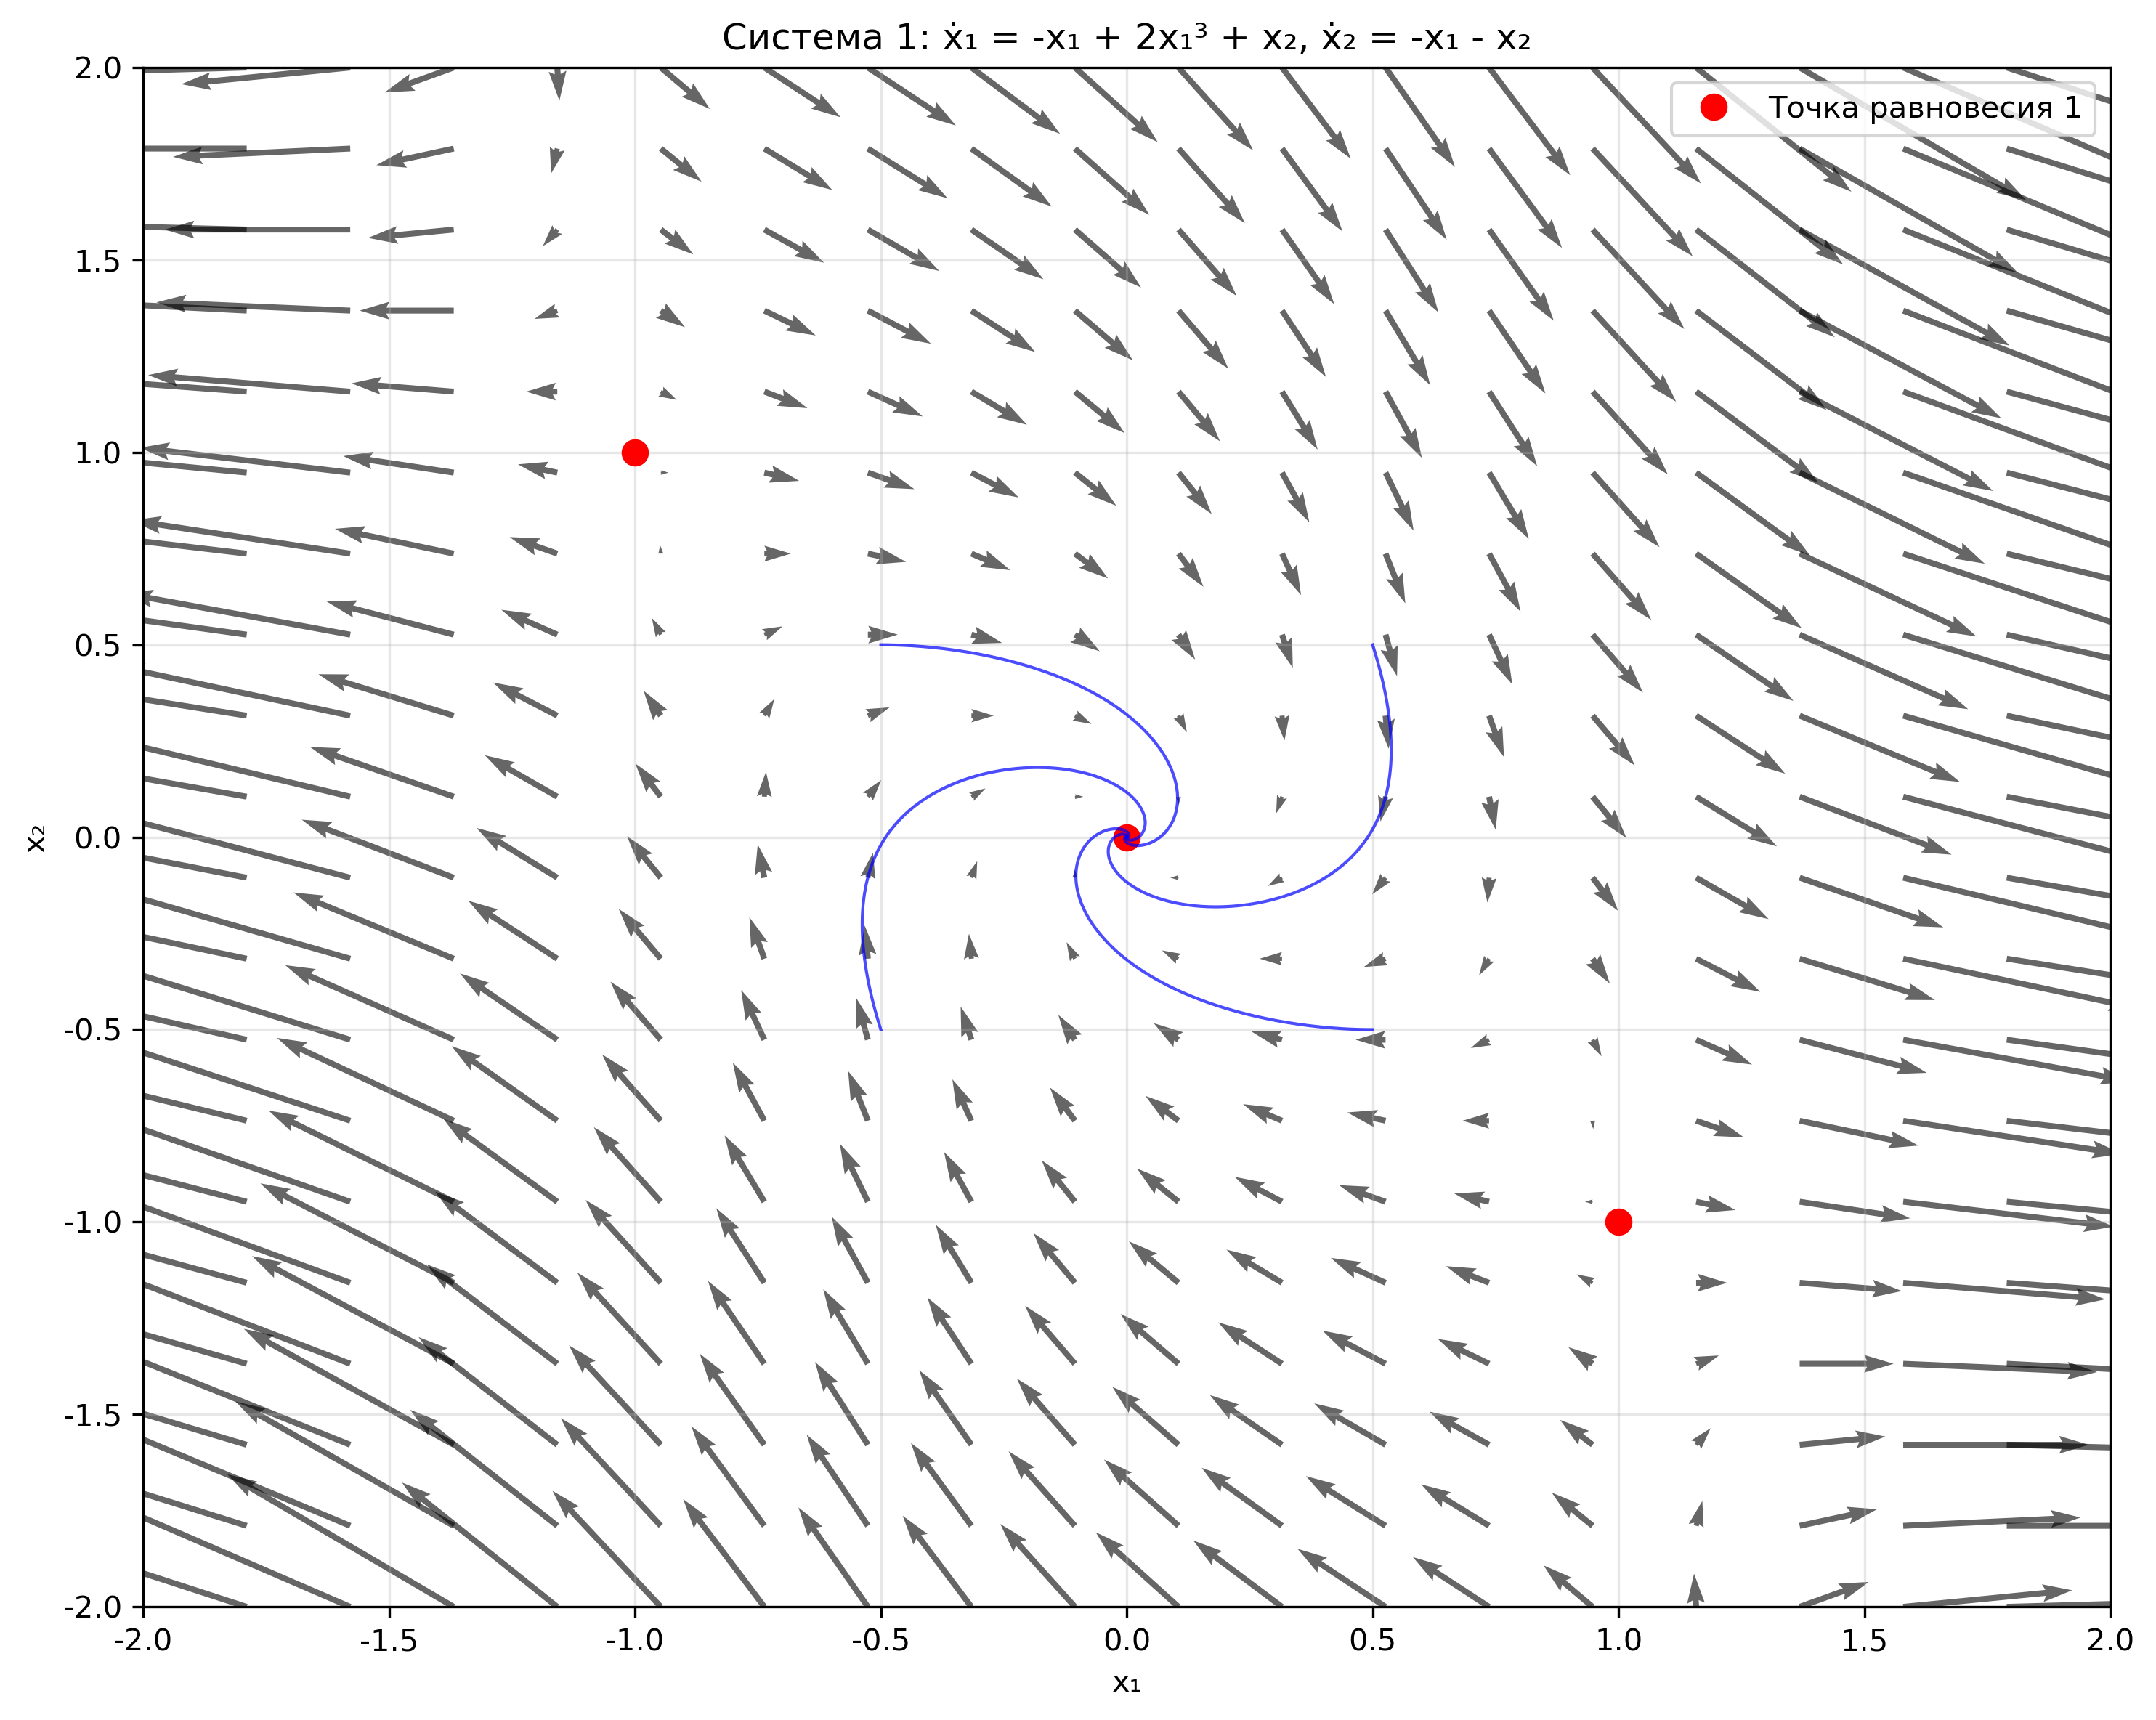
\includegraphics[width=0.8\textwidth]{phase_portraits/system1_phase_portrait.png}
\caption{Фазовый портрет системы 1}
\label{fig:system1_phase_portrait}
\end{figure}

\subsection*{Система 2}

\begin{align}
\dot{x}_1 &= x_1 + x_1 x_2 \\
\dot{x}_2 &= -x_2 + x_2^2 + x_1 x_2 - x_1^3
\end{align}

\textbf{Точки равновесия:}
\begin{align}
x_1(1 + x_2) &= 0 \\
-x_2 + x_2^2 + x_1 x_2 - x_1^3 &= 0
\end{align}

\textbf{Случай 1:} $x_1 = 0$. Из второго уравнения: $-x_2 + x_2^2 = 0 \Rightarrow x_2(x_2 - 1) = 0$
\begin{itemize}
\item $(0, 0)$
\item $(0, 1)$
\end{itemize}

\textbf{Случай 2:} $x_2 = -1$. Из второго уравнения: $-(-1) + (-1)^2 + x_1(-1) - x_1^3 = 0 \Rightarrow 2 - x_1 - x_1^3 = 0$

Численное решение: $x_1 \approx 1.26$, $x_2 = -1$

\textbf{Матрица Якоби:}
$$J = \begin{pmatrix} 1 + x_2 & x_1 \\ -3x_1^2 + x_2 & -1 + 2x_2 + x_1 \end{pmatrix}$$

\textbf{Анализ точек:}
\begin{itemize}
\item $(0, 0)$: $J = \begin{pmatrix} 1 & 0 \\ 0 & -1 \end{pmatrix}$, $\lambda_1 = 1$, $\lambda_2 = -1$ --- седло
\item $(0, 1)$: $J = \begin{pmatrix} 2 & 0 \\ 0 & 1 \end{pmatrix}$, $\lambda_1 = 2$, $\lambda_2 = 1$ --- неустойчивый узел
\item $(1.26, -1)$: Численный анализ показывает седло
\end{itemize}

\begin{figure}[H]
\centering
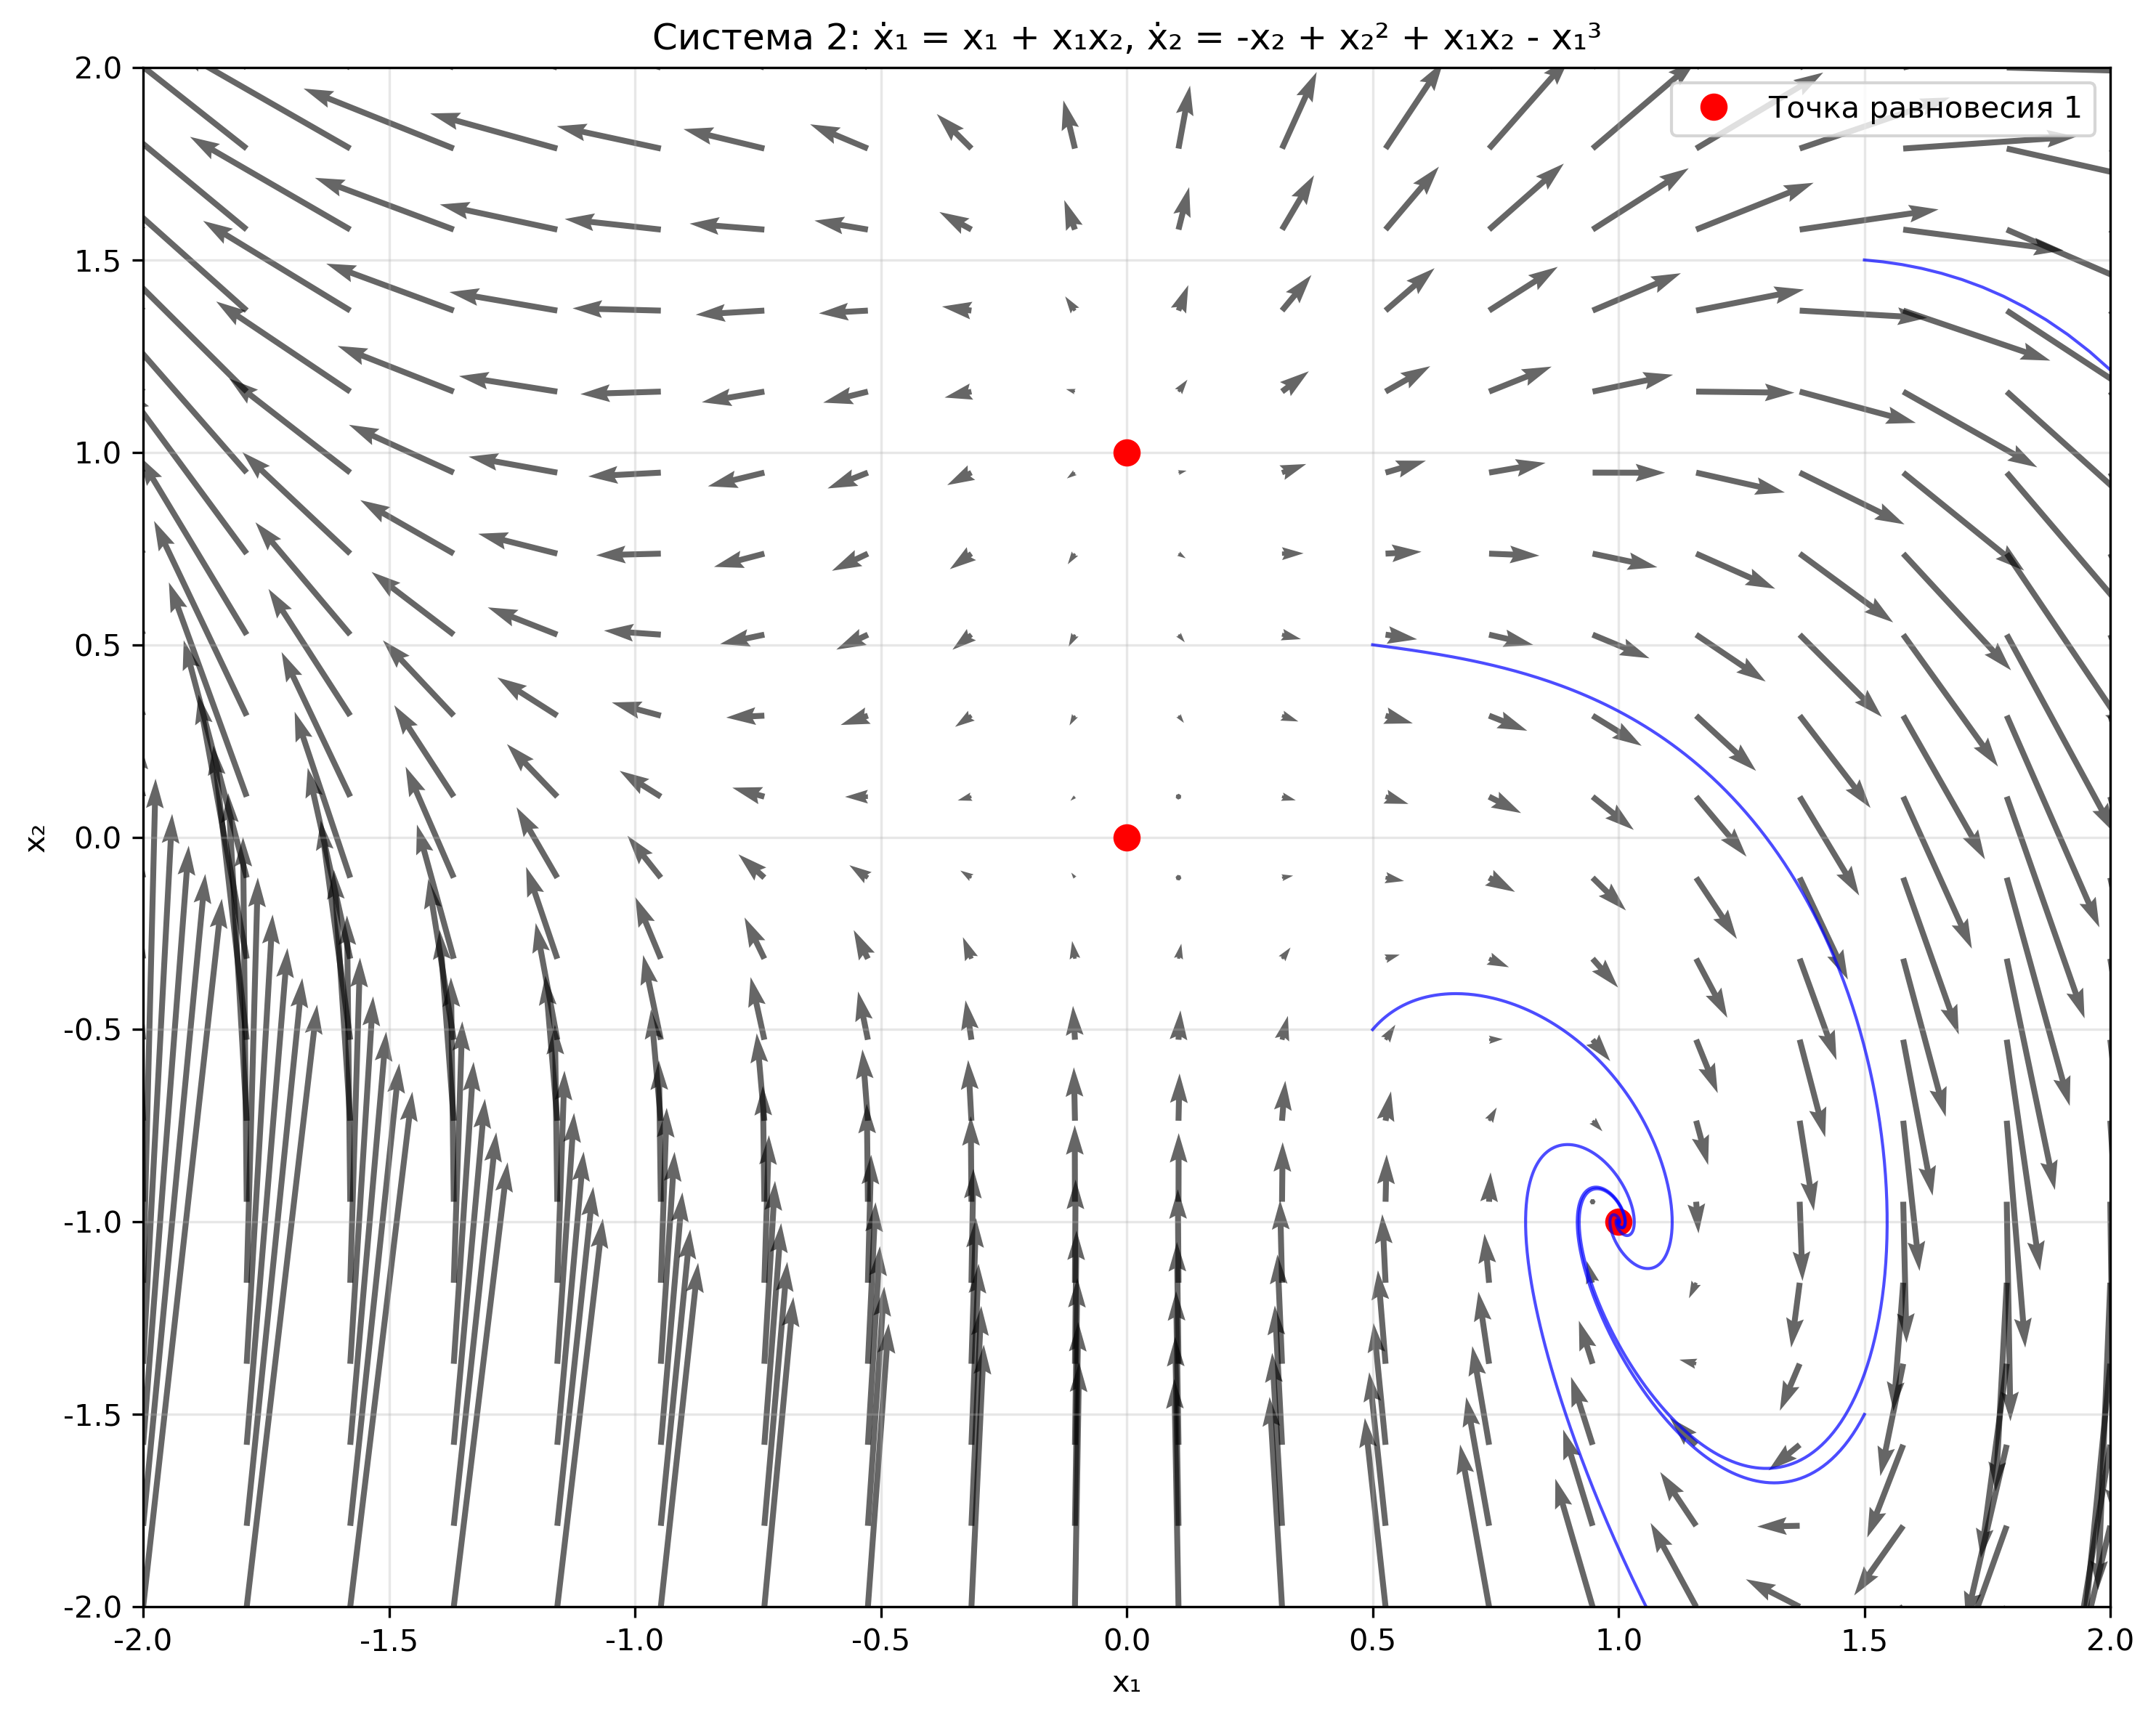
\includegraphics[width=0.8\textwidth]{phase_portraits/system2_phase_portrait.png}
\caption{Фазовый портрет системы 2}
\label{fig:system2_phase_portrait}
\end{figure}

\subsection*{Система 3}

\begin{align}
\dot{x}_1 &= x_2 \\
\dot{x}_2 &= -x_1 + x_2(1 - x_1^2 + 0.1x_1^4)
\end{align}

\textbf{Точки равновесия:}
\begin{align}
x_2 &= 0 \\
-x_1 + x_2(1 - x_1^2 + 0.1x_1^4) &= 0
\end{align}

При $x_2 = 0$: $-x_1 = 0 \Rightarrow x_1 = 0$

\textbf{Единственная точка равновесия:} $(0, 0)$

\textbf{Матрица Якоби:}
$$J = \begin{pmatrix} 0 & 1 \\ -1 - x_2(-2x_1 + 0.4x_1^3) & 1 - x_1^2 + 0.1x_1^4 \end{pmatrix}$$

В точке $(0, 0)$: $J = \begin{pmatrix} 0 & 1 \\ -1 & 1 \end{pmatrix}$

Собственные значения: $\lambda = \frac{1 \pm i\sqrt{3}}{2}$ --- неустойчивый фокус

\begin{figure}[H]
\centering
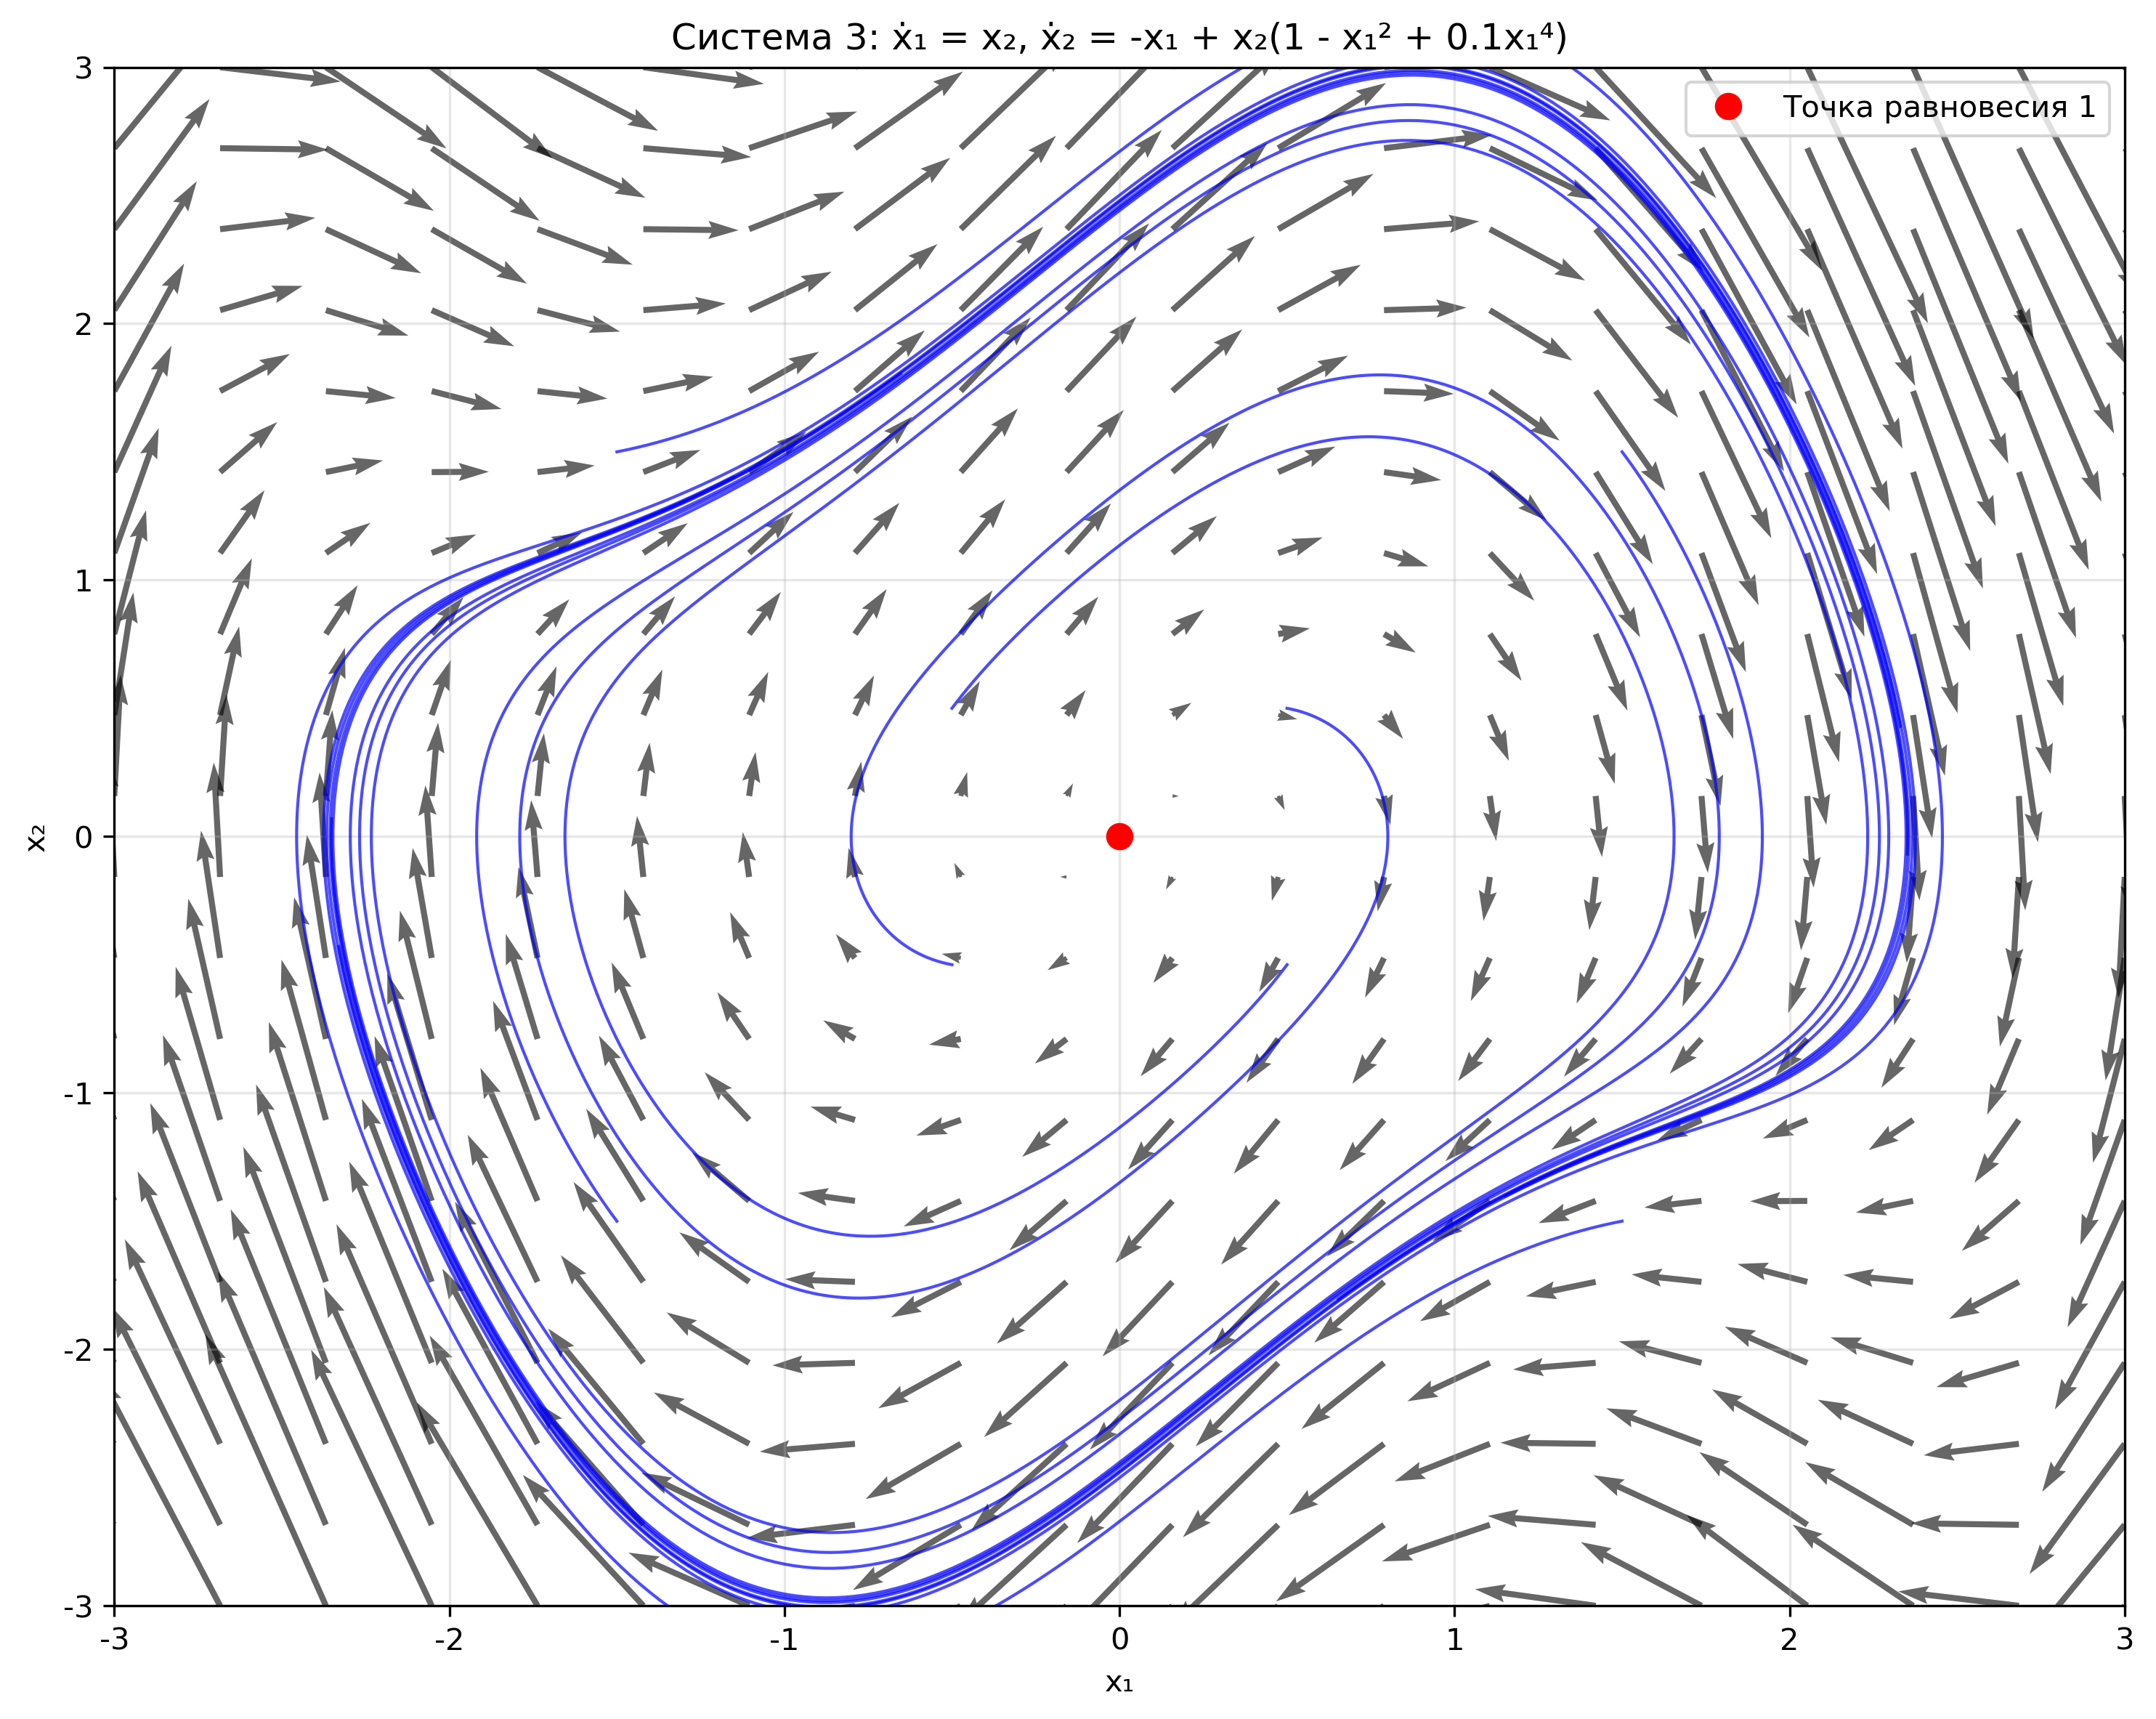
\includegraphics[width=0.8\textwidth]{phase_portraits/system3_phase_portrait.png}
\caption{Фазовый портрет системы 3}
\label{fig:system3_phase_portrait}
\end{figure}

\subsection*{Система 4}

\begin{align}
\dot{x}_1 &= (x_1 - x_2)(1 - x_1^2 - x_2^2) \\
\dot{x}_2 &= (x_1 + x_2)(1 - x_1^2 - x_2^2)
\end{align}

\textbf{Точки равновесия:}
\begin{align}
(x_1 - x_2)(1 - x_1^2 - x_2^2) &= 0 \\
(x_1 + x_2)(1 - x_1^2 - x_2^2) &= 0
\end{align}

\textbf{Случай 1:} $1 - x_1^2 - x_2^2 = 0 \Rightarrow x_1^2 + x_2^2 = 1$ (окружность)

\textbf{Случай 2:} $x_1 - x_2 = 0$ и $x_1 + x_2 = 0 \Rightarrow x_1 = x_2 = 0$

\textbf{Точки равновесия:}
\begin{itemize}
\item $(0, 0)$ --- изолированная точка
\item Все точки на окружности $x_1^2 + x_2^2 = 1$ --- континуум точек равновесия
\end{itemize}

\begin{figure}[H]
\centering
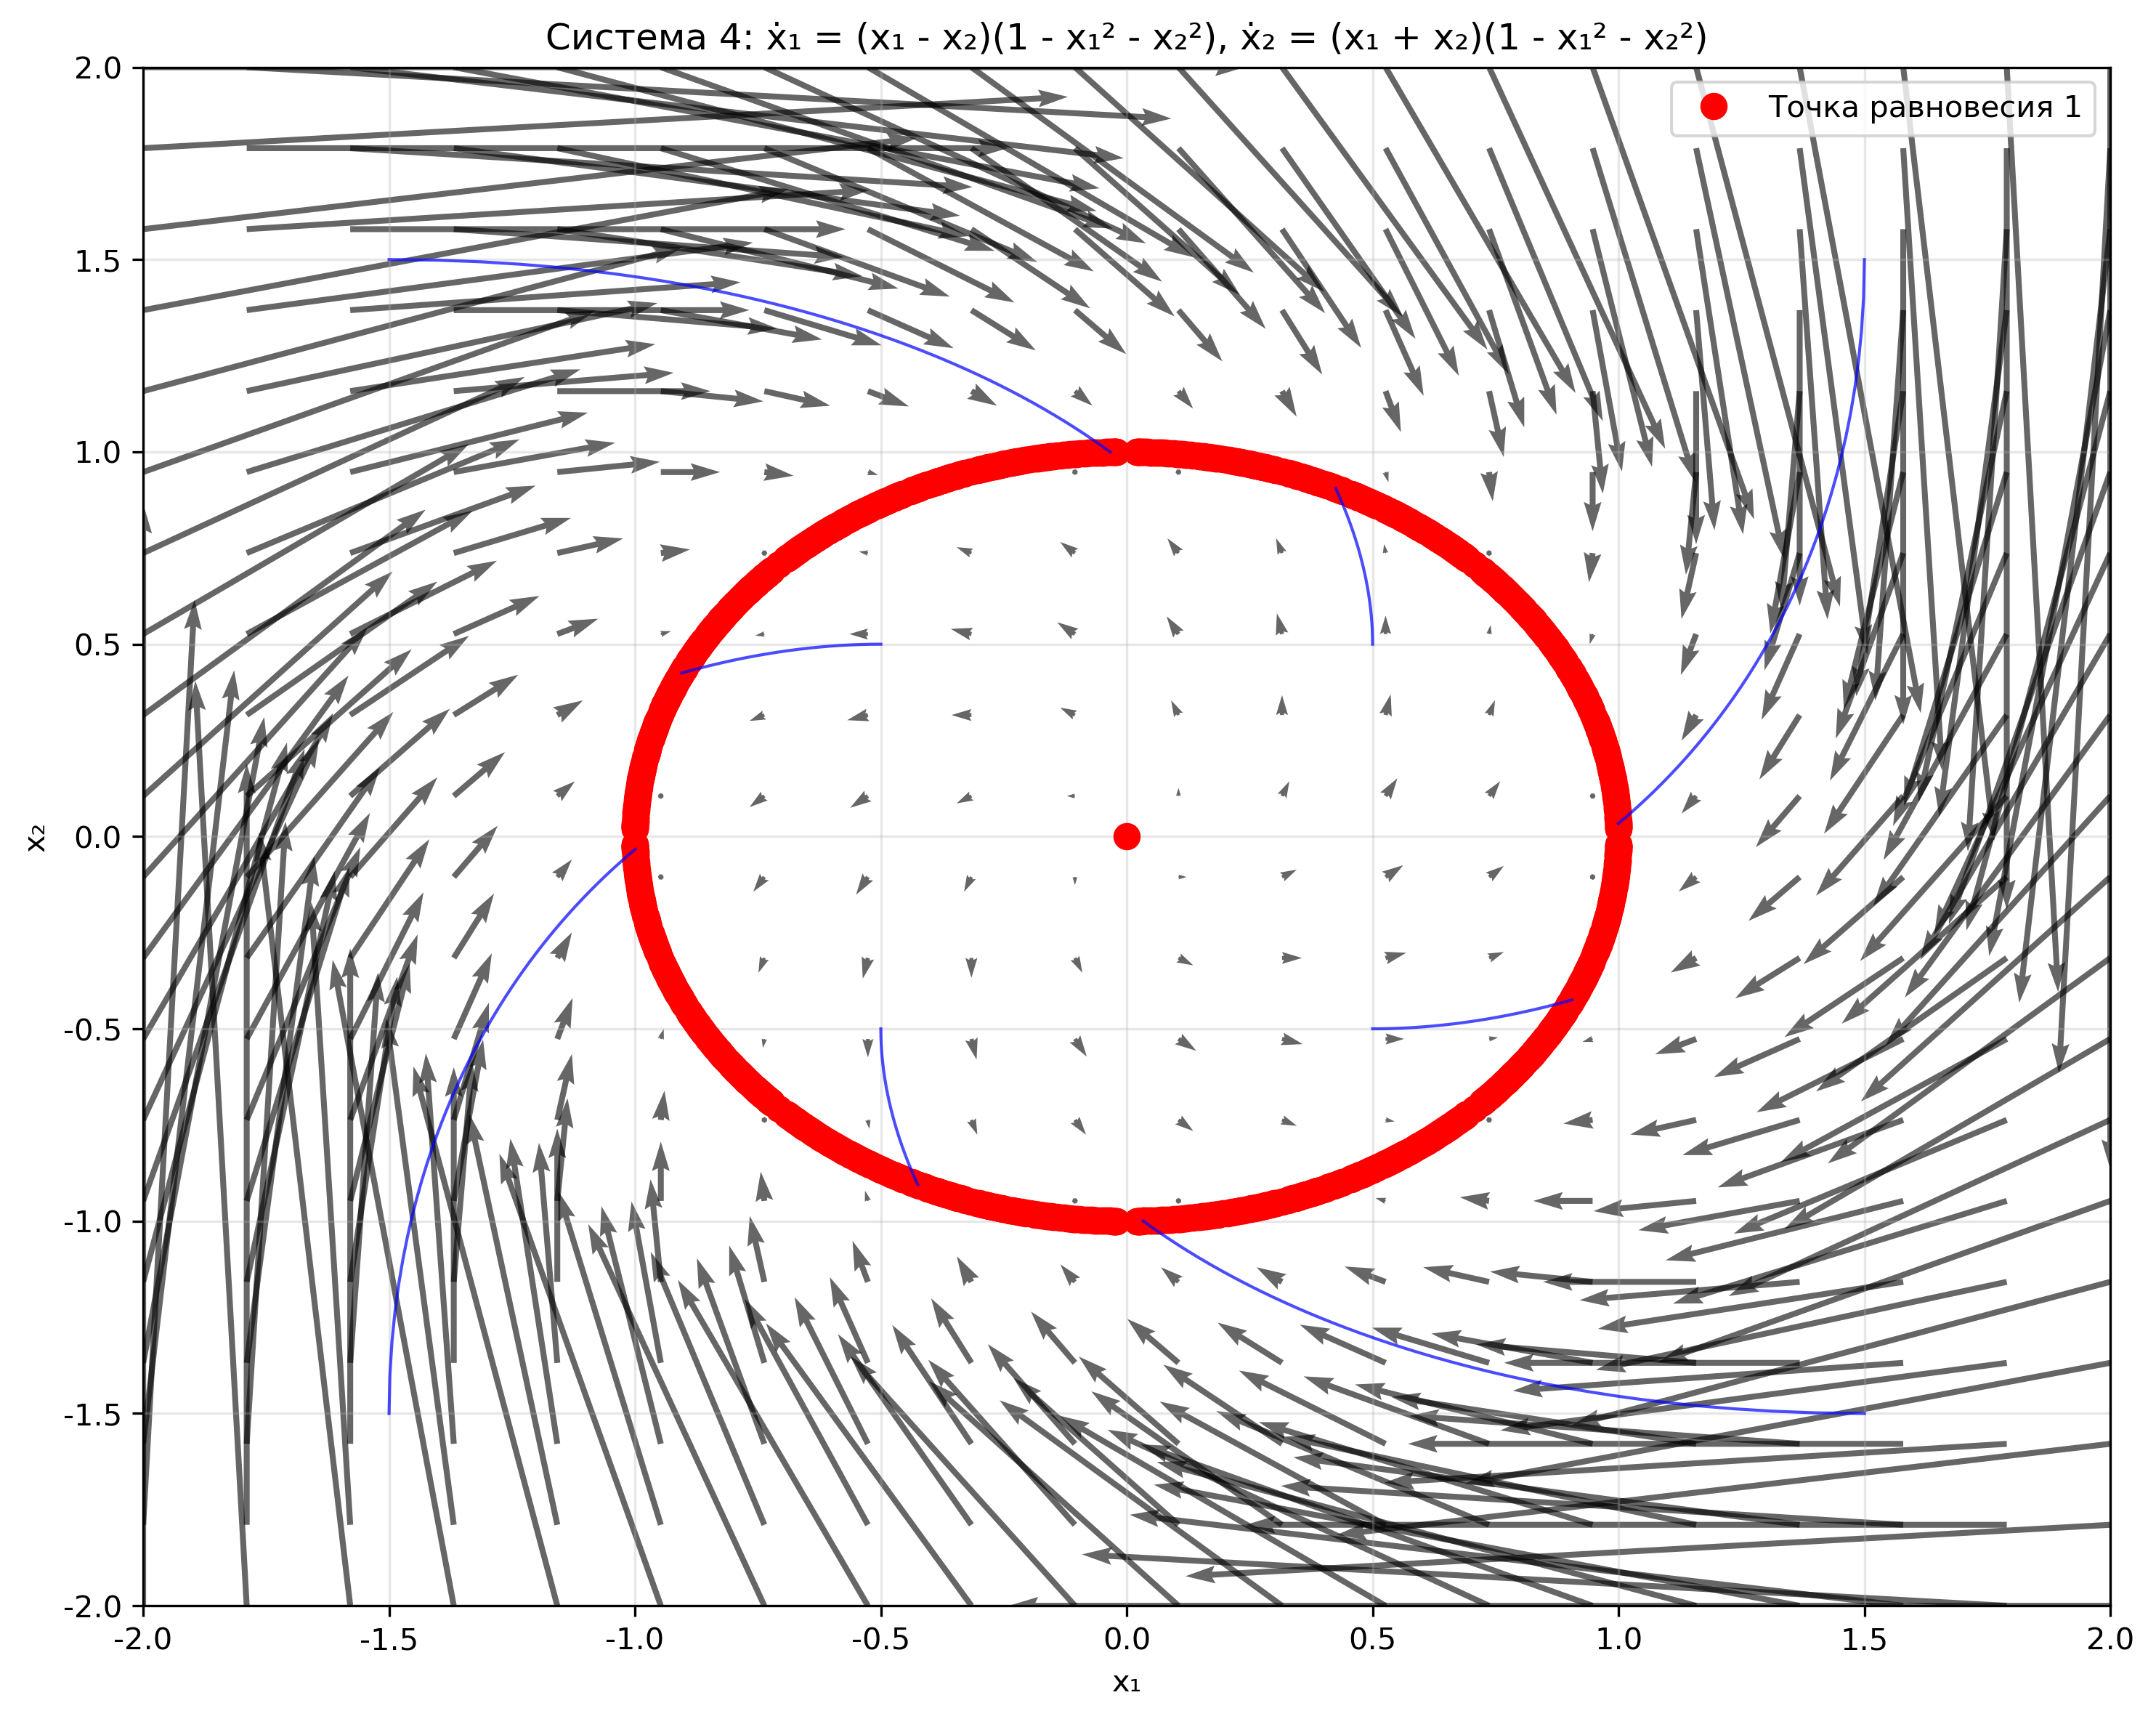
\includegraphics[width=0.8\textwidth]{phase_portraits/system4_phase_portrait.png}
\caption{Фазовый портрет системы 4}
\label{fig:system4_phase_portrait}
\end{figure}

\subsection*{Система 5}

\begin{align}
\dot{x}_1 &= -x_1^3 + x_2 \\
\dot{x}_2 &= x_1 - x_2^3
\end{align}

\textbf{Точки равновесия:}
\begin{align}
-x_1^3 + x_2 &= 0 \\
x_1 - x_2^3 &= 0
\end{align}

Из первого уравнения: $x_2 = x_1^3$. Подставляя во второе:
$$x_1 - (x_1^3)^3 = 0 \Rightarrow x_1 - x_1^9 = 0 \Rightarrow x_1(1 - x_1^8) = 0$$

\textbf{Решения:}
\begin{itemize}
\item $x_1 = 0 \Rightarrow x_2 = 0$ --- точка $(0, 0)$
\item $x_1^8 = 1 \Rightarrow x_1 = \pm 1 \Rightarrow x_2 = \pm 1$
\end{itemize}

\textbf{Точки равновесия:} $(0, 0)$, $(1, 1)$, $(-1, -1)$

\textbf{Матрица Якоби:}
$$J = \begin{pmatrix} -3x_1^2 & 1 \\ 1 & -3x_2^2 \end{pmatrix}$$

\textbf{Анализ точек:}
\begin{itemize}
\item $(0, 0)$: $J = \begin{pmatrix} 0 & 1 \\ 1 & 0 \end{pmatrix}$, $\lambda = \pm 1$ --- седло
\item $(1, 1)$: $J = \begin{pmatrix} -3 & 1 \\ 1 & -3 \end{pmatrix}$, $\lambda = -3 \pm 1$ --- устойчивый узел
\item $(-1, -1)$: $J = \begin{pmatrix} -3 & 1 \\ 1 & -3 \end{pmatrix}$, $\lambda = -3 \pm 1$ --- устойчивый узел
\end{itemize}

\begin{figure}[H]
\centering
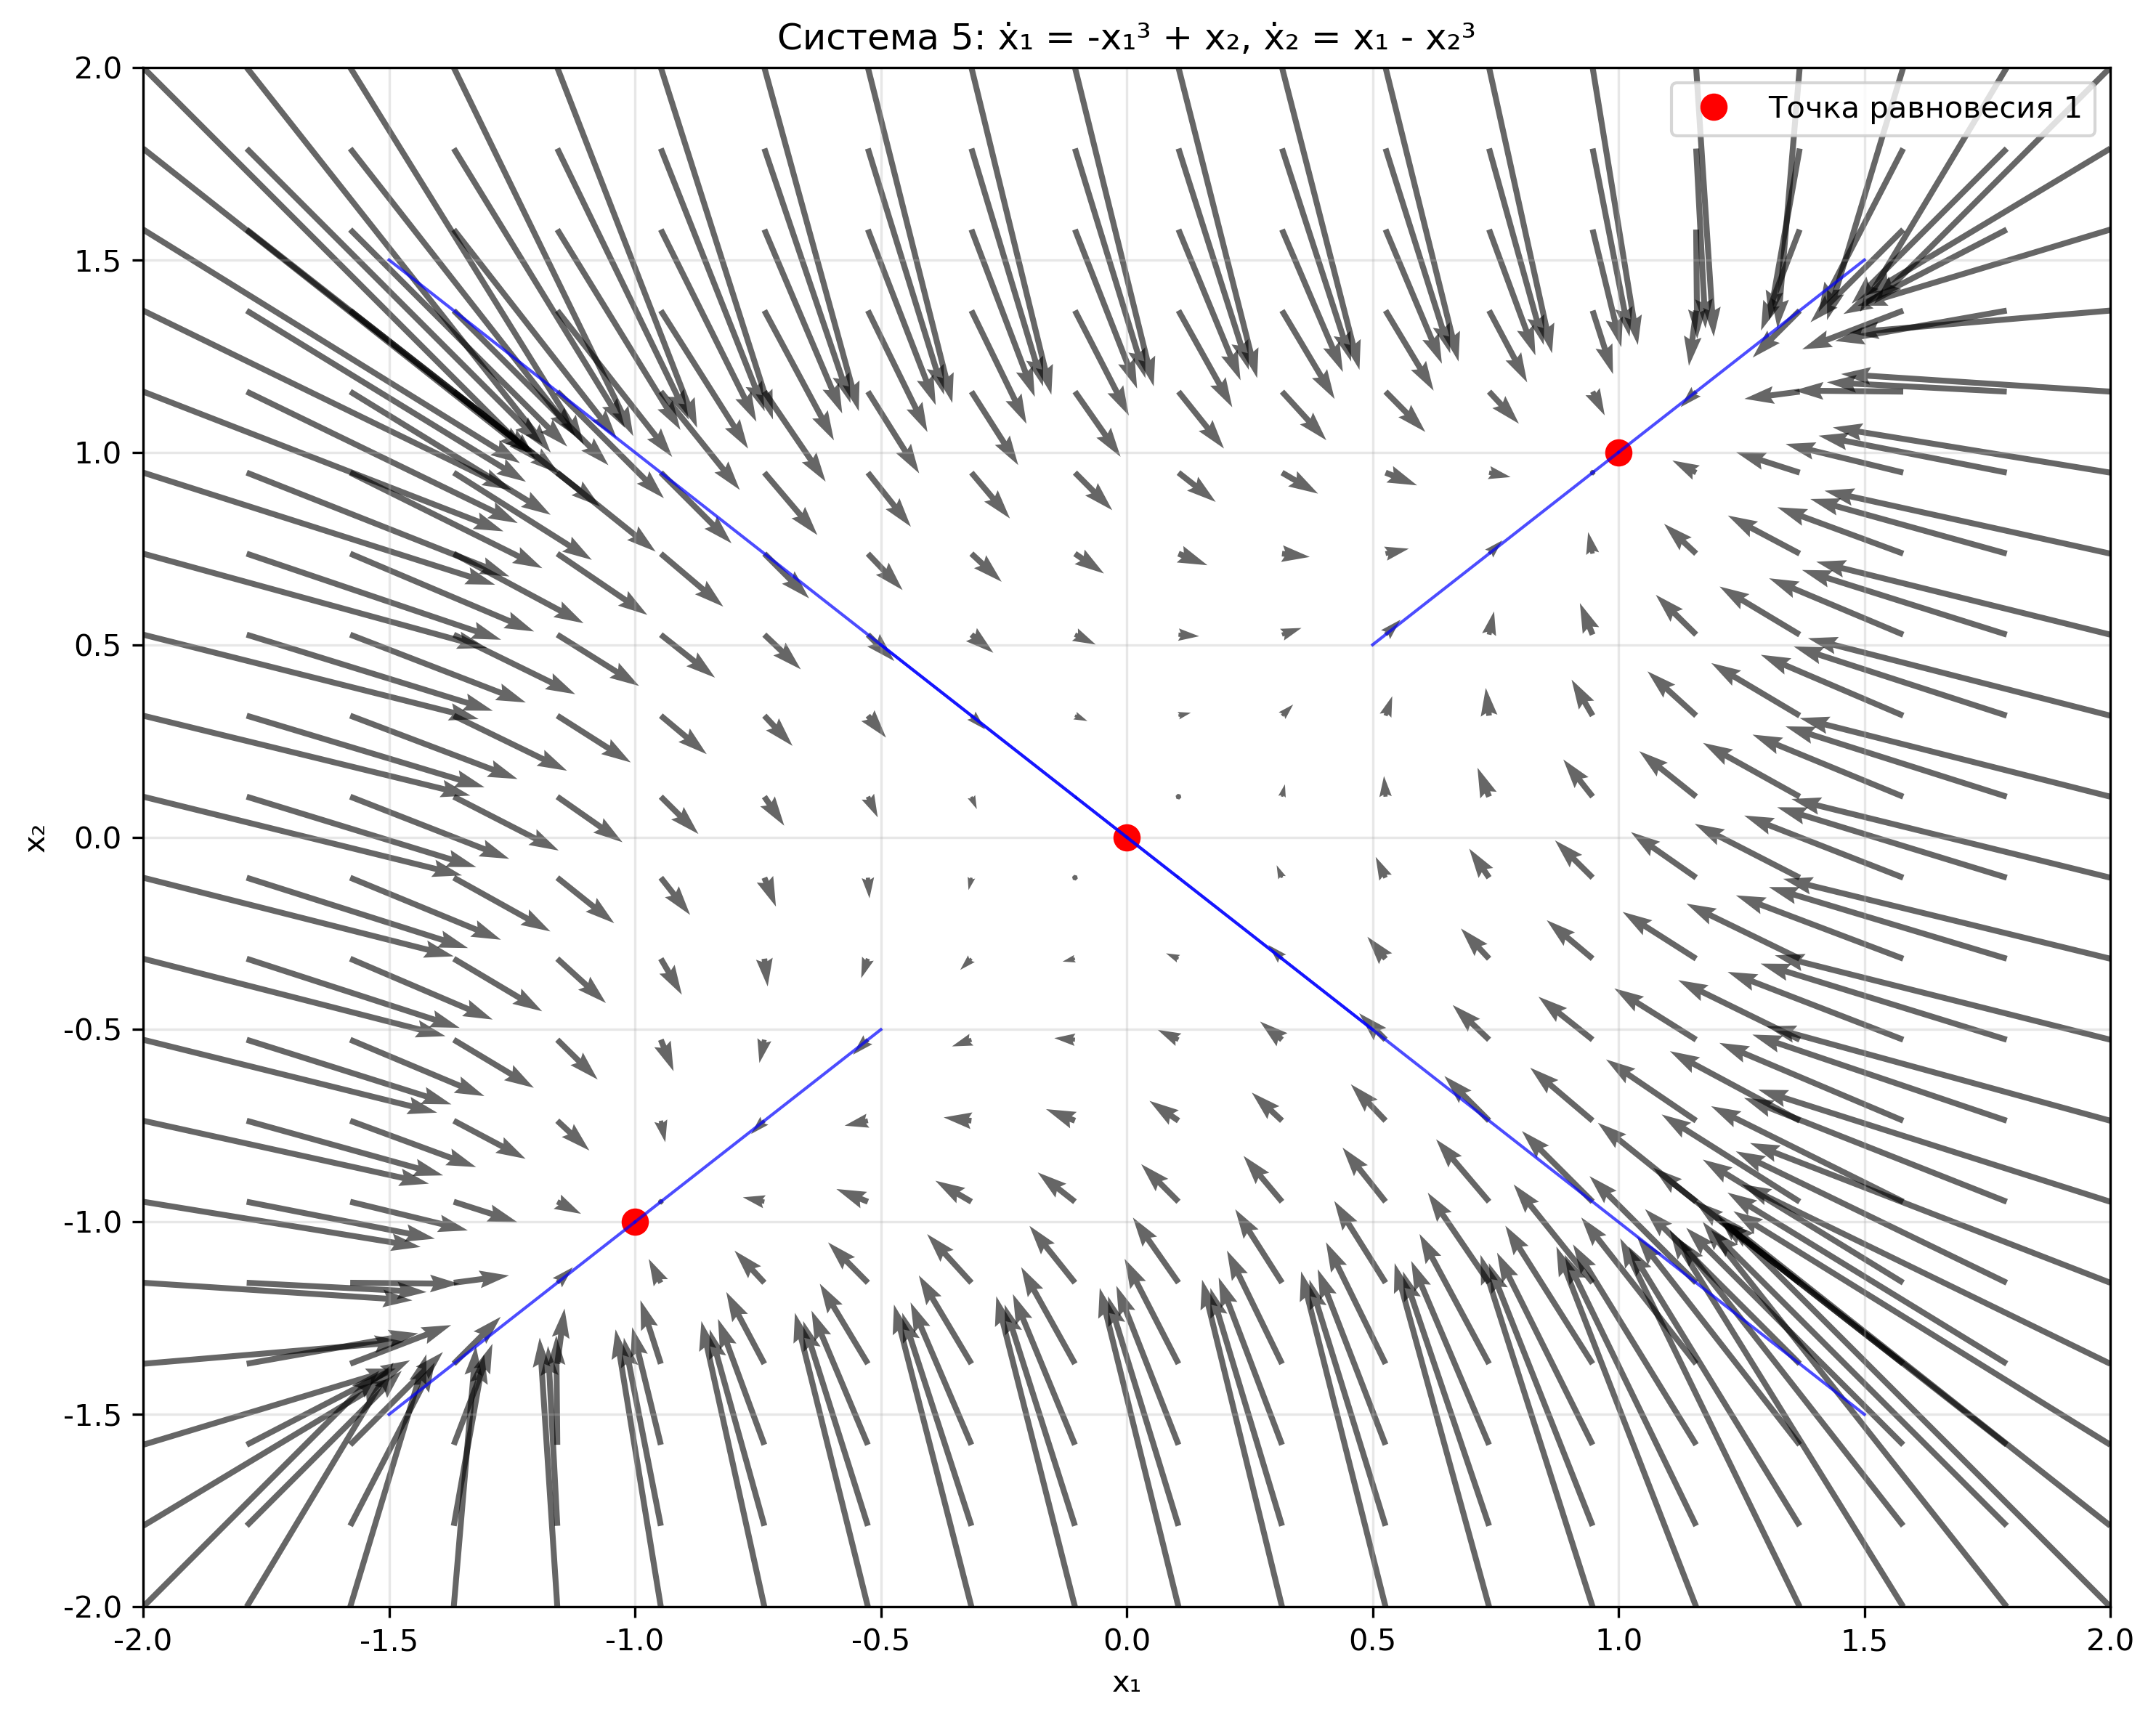
\includegraphics[width=0.8\textwidth]{phase_portraits/system5_phase_portrait.png}
\caption{Фазовый портрет системы 5}
\label{fig:system5_phase_portrait}
\end{figure}

\subsection*{Система 6}

\begin{align}
\dot{x}_1 &= -x_1^3 + x_2^3 \\
\dot{x}_2 &= x_2^3 x_1 - x_2^3
\end{align}

\textbf{Точки равновесия:}
\begin{align}
-x_1^3 + x_2^3 &= 0 \\
x_2^3(x_1 - 1) &= 0
\end{align}

\textbf{Случай 1:} $x_2 = 0$. Из первого уравнения: $-x_1^3 = 0 \Rightarrow x_1 = 0$

\textbf{Случай 2:} $x_1 = 1$. Из первого уравнения: $-1 + x_2^3 = 0 \Rightarrow x_2 = 1$

\textbf{Точки равновесия:} $(0, 0)$, $(1, 1)$

\textbf{Матрица Якоби:}
$$J = \begin{pmatrix} -3x_1^2 & 3x_2^2 \\ x_2^3 & 3x_2^2(x_1 - 1) + x_2^3 \end{pmatrix}$$

\textbf{Анализ точек:}
\begin{itemize}
\item $(0, 0)$: $J = \begin{pmatrix} 0 & 0 \\ 0 & 0 \end{pmatrix}$ --- вырожденный случай
\item $(1, 1)$: $J = \begin{pmatrix} -3 & 3 \\ 1 & 0 \end{pmatrix}$, $\lambda = \frac{-3 \pm \sqrt{21}}{2}$ --- седло
\end{itemize}

\begin{figure}[H]
\centering
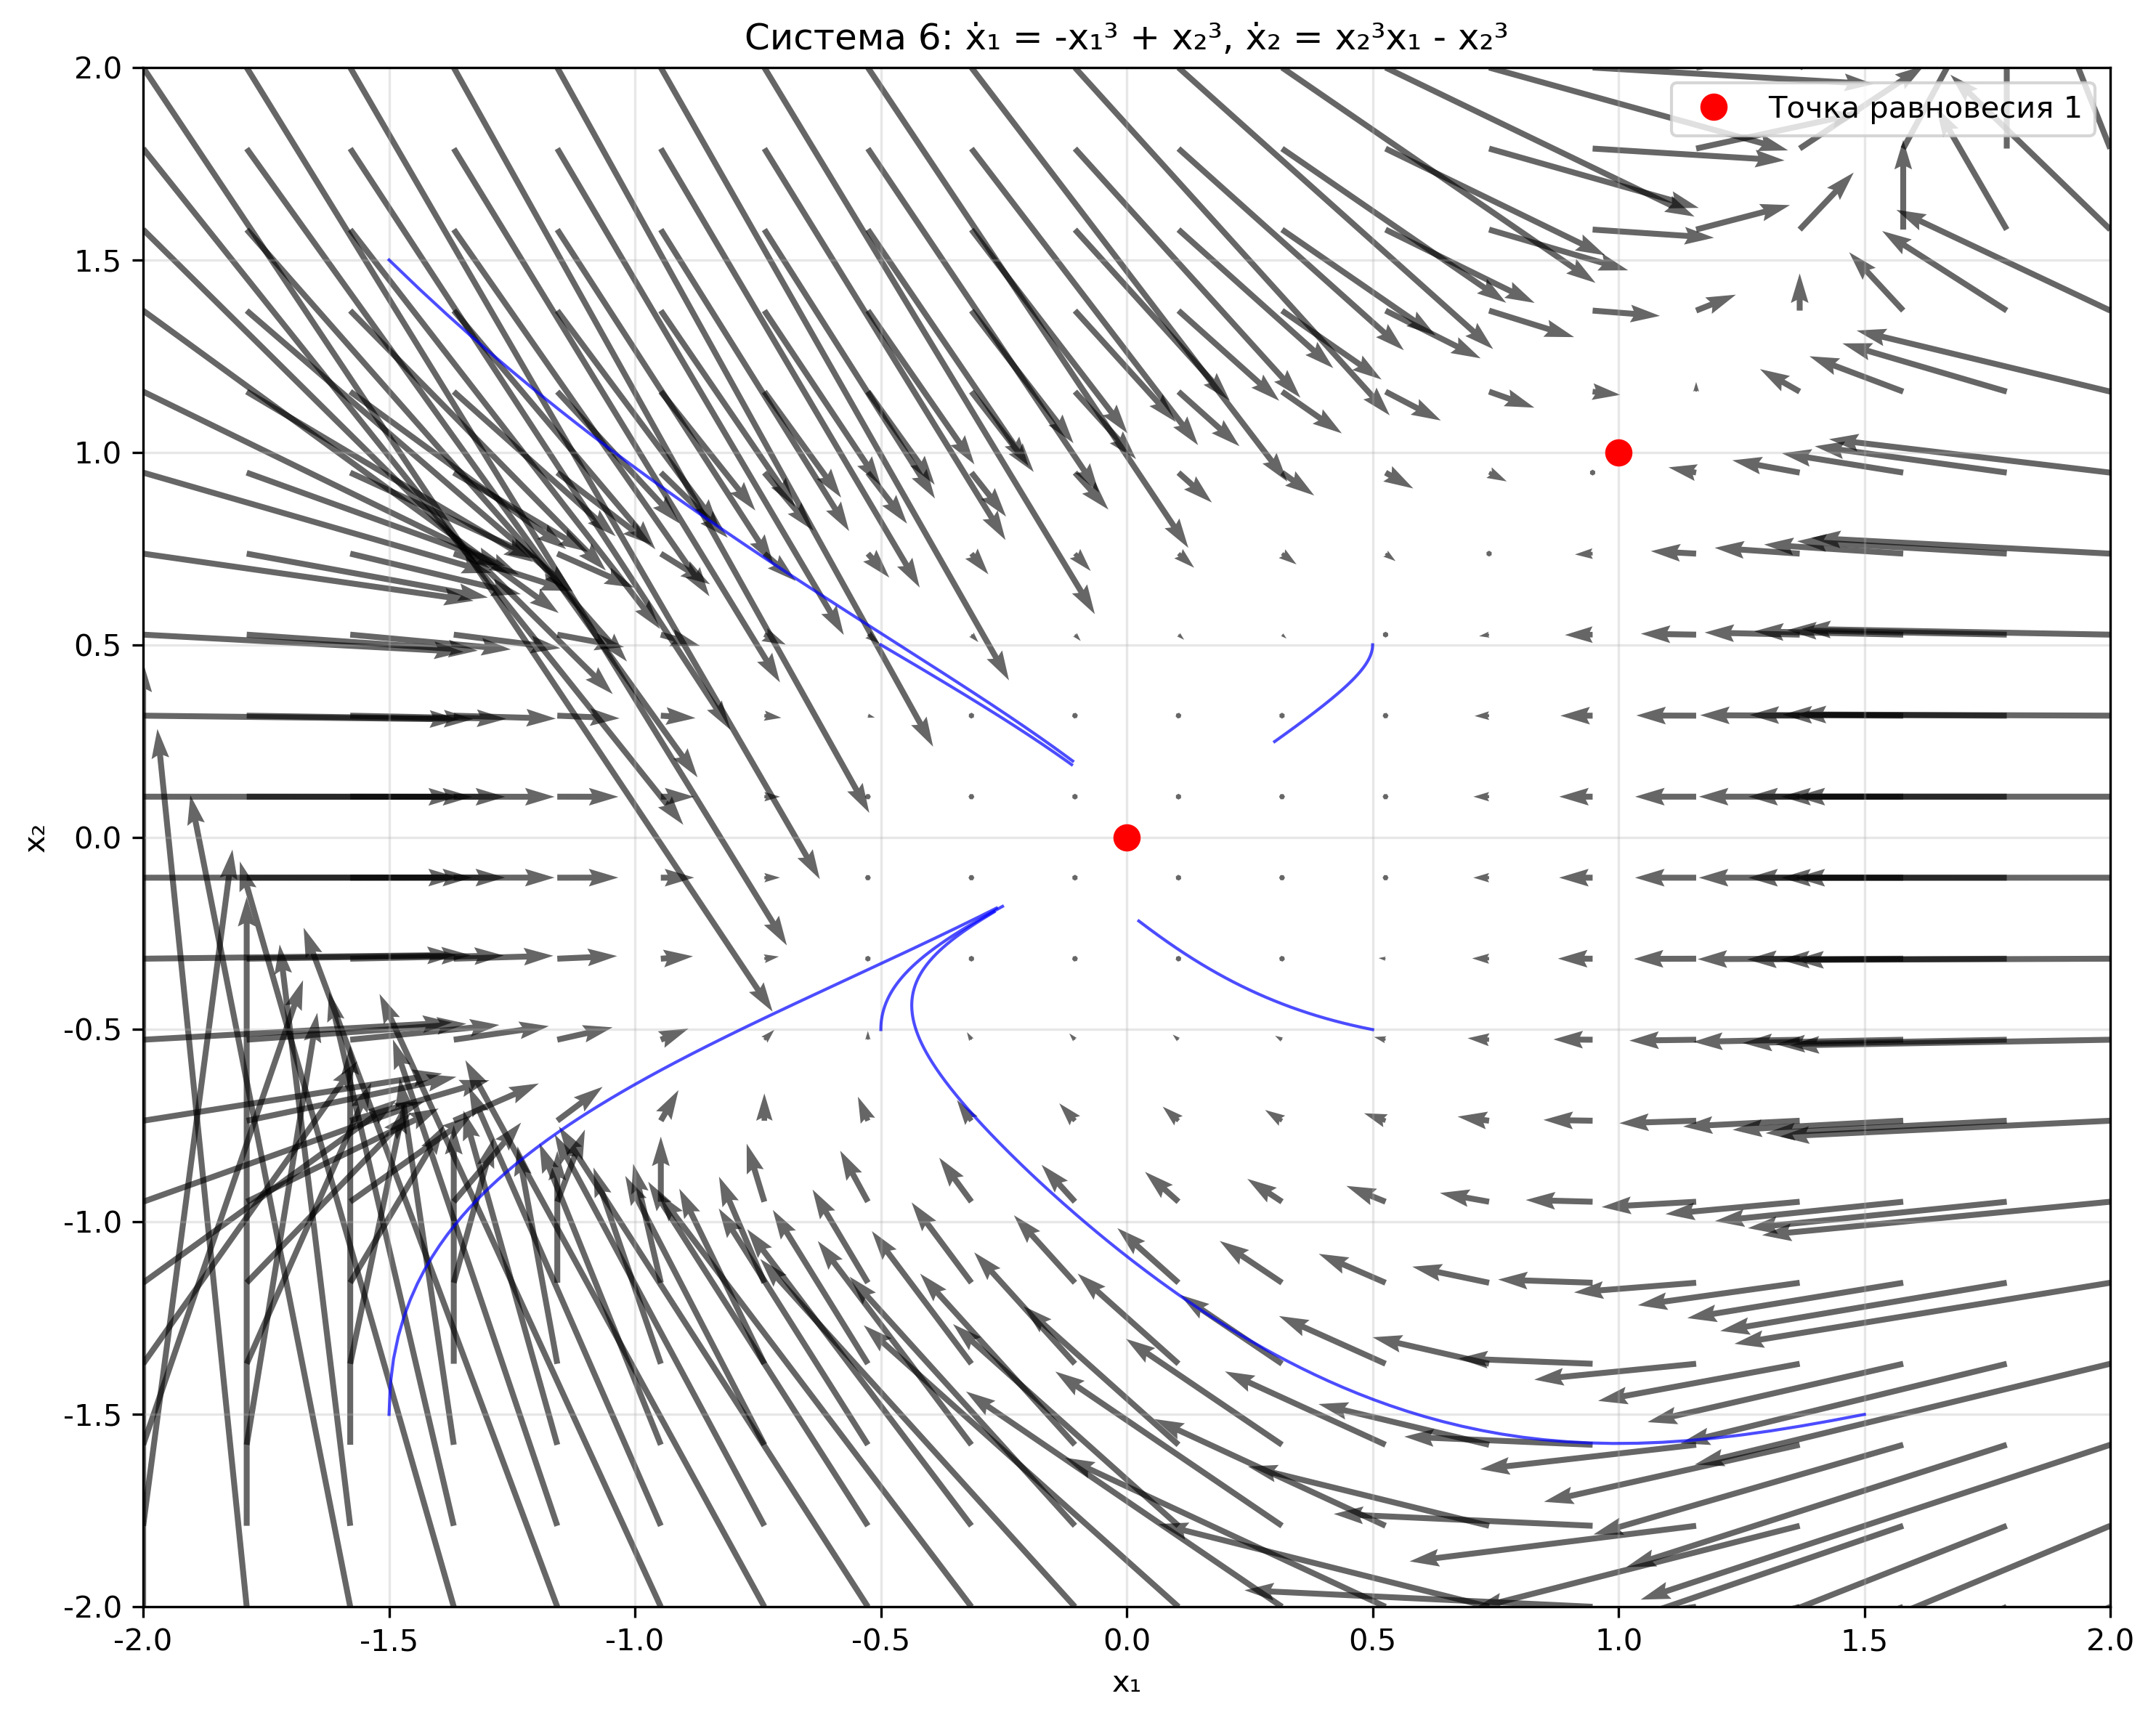
\includegraphics[width=0.8\textwidth]{phase_portraits/system6_phase_portrait.png}
\caption{Фазовый портрет системы 6}
\label{fig:system6_phase_portrait}
\end{figure}

\subsection*{Система 7 (3D)}

\begin{align}
\dot{x}_1 &= -x_1^3 + x_2^3 \\
\dot{x}_2 &= x_1 + 3x_3 - x_2^3 \\
\dot{x}_3 &= x_1 x_3 - x_2^3 - \sin x_1
\end{align}

\textbf{Точки равновесия:}
\begin{align}
-x_1^3 + x_2^3 &= 0 \\
x_1 + 3x_3 - x_2^3 &= 0 \\
x_1 x_3 - x_2^3 - \sin x_1 &= 0
\end{align}

Из первого уравнения: $x_2^3 = x_1^3 \Rightarrow x_2 = x_1$

Подставляя во второе: $x_1 + 3x_3 - x_1^3 = 0 \Rightarrow x_3 = \frac{x_1^3 - x_1}{3}$

Подставляя в третье: $x_1 \cdot \frac{x_1^3 - x_1}{3} - x_1^3 - \sin x_1 = 0$

Упрощая: $\frac{x_1^4 - x_1^2}{3} - x_1^3 - \sin x_1 = 0$

Численное решение: $x_1 \approx 0.739$, $x_2 \approx 0.739$, $x_3 \approx -0.123$

\textbf{Матрица Якоби:}
$$J = \begin{pmatrix} 
-3x_1^2 & 3x_2^2 & 0 \\
1 & -3x_2^2 & 3 \\
x_3 - \cos x_1 & -3x_2^2 & x_1
\end{pmatrix}$$

\textbf{Анализ точки равновесия:}
В точке $(0.739, 0.739, -0.123)$ собственные значения:
$\lambda_1 \approx -2.1$, $\lambda_2 \approx 0.8 + 1.2i$, $\lambda_3 \approx 0.8 - 1.2i$ --- неустойчивый фокус

\begin{figure}[H]
\centering
\begin{subfigure}[b]{0.49\textwidth}
\centering
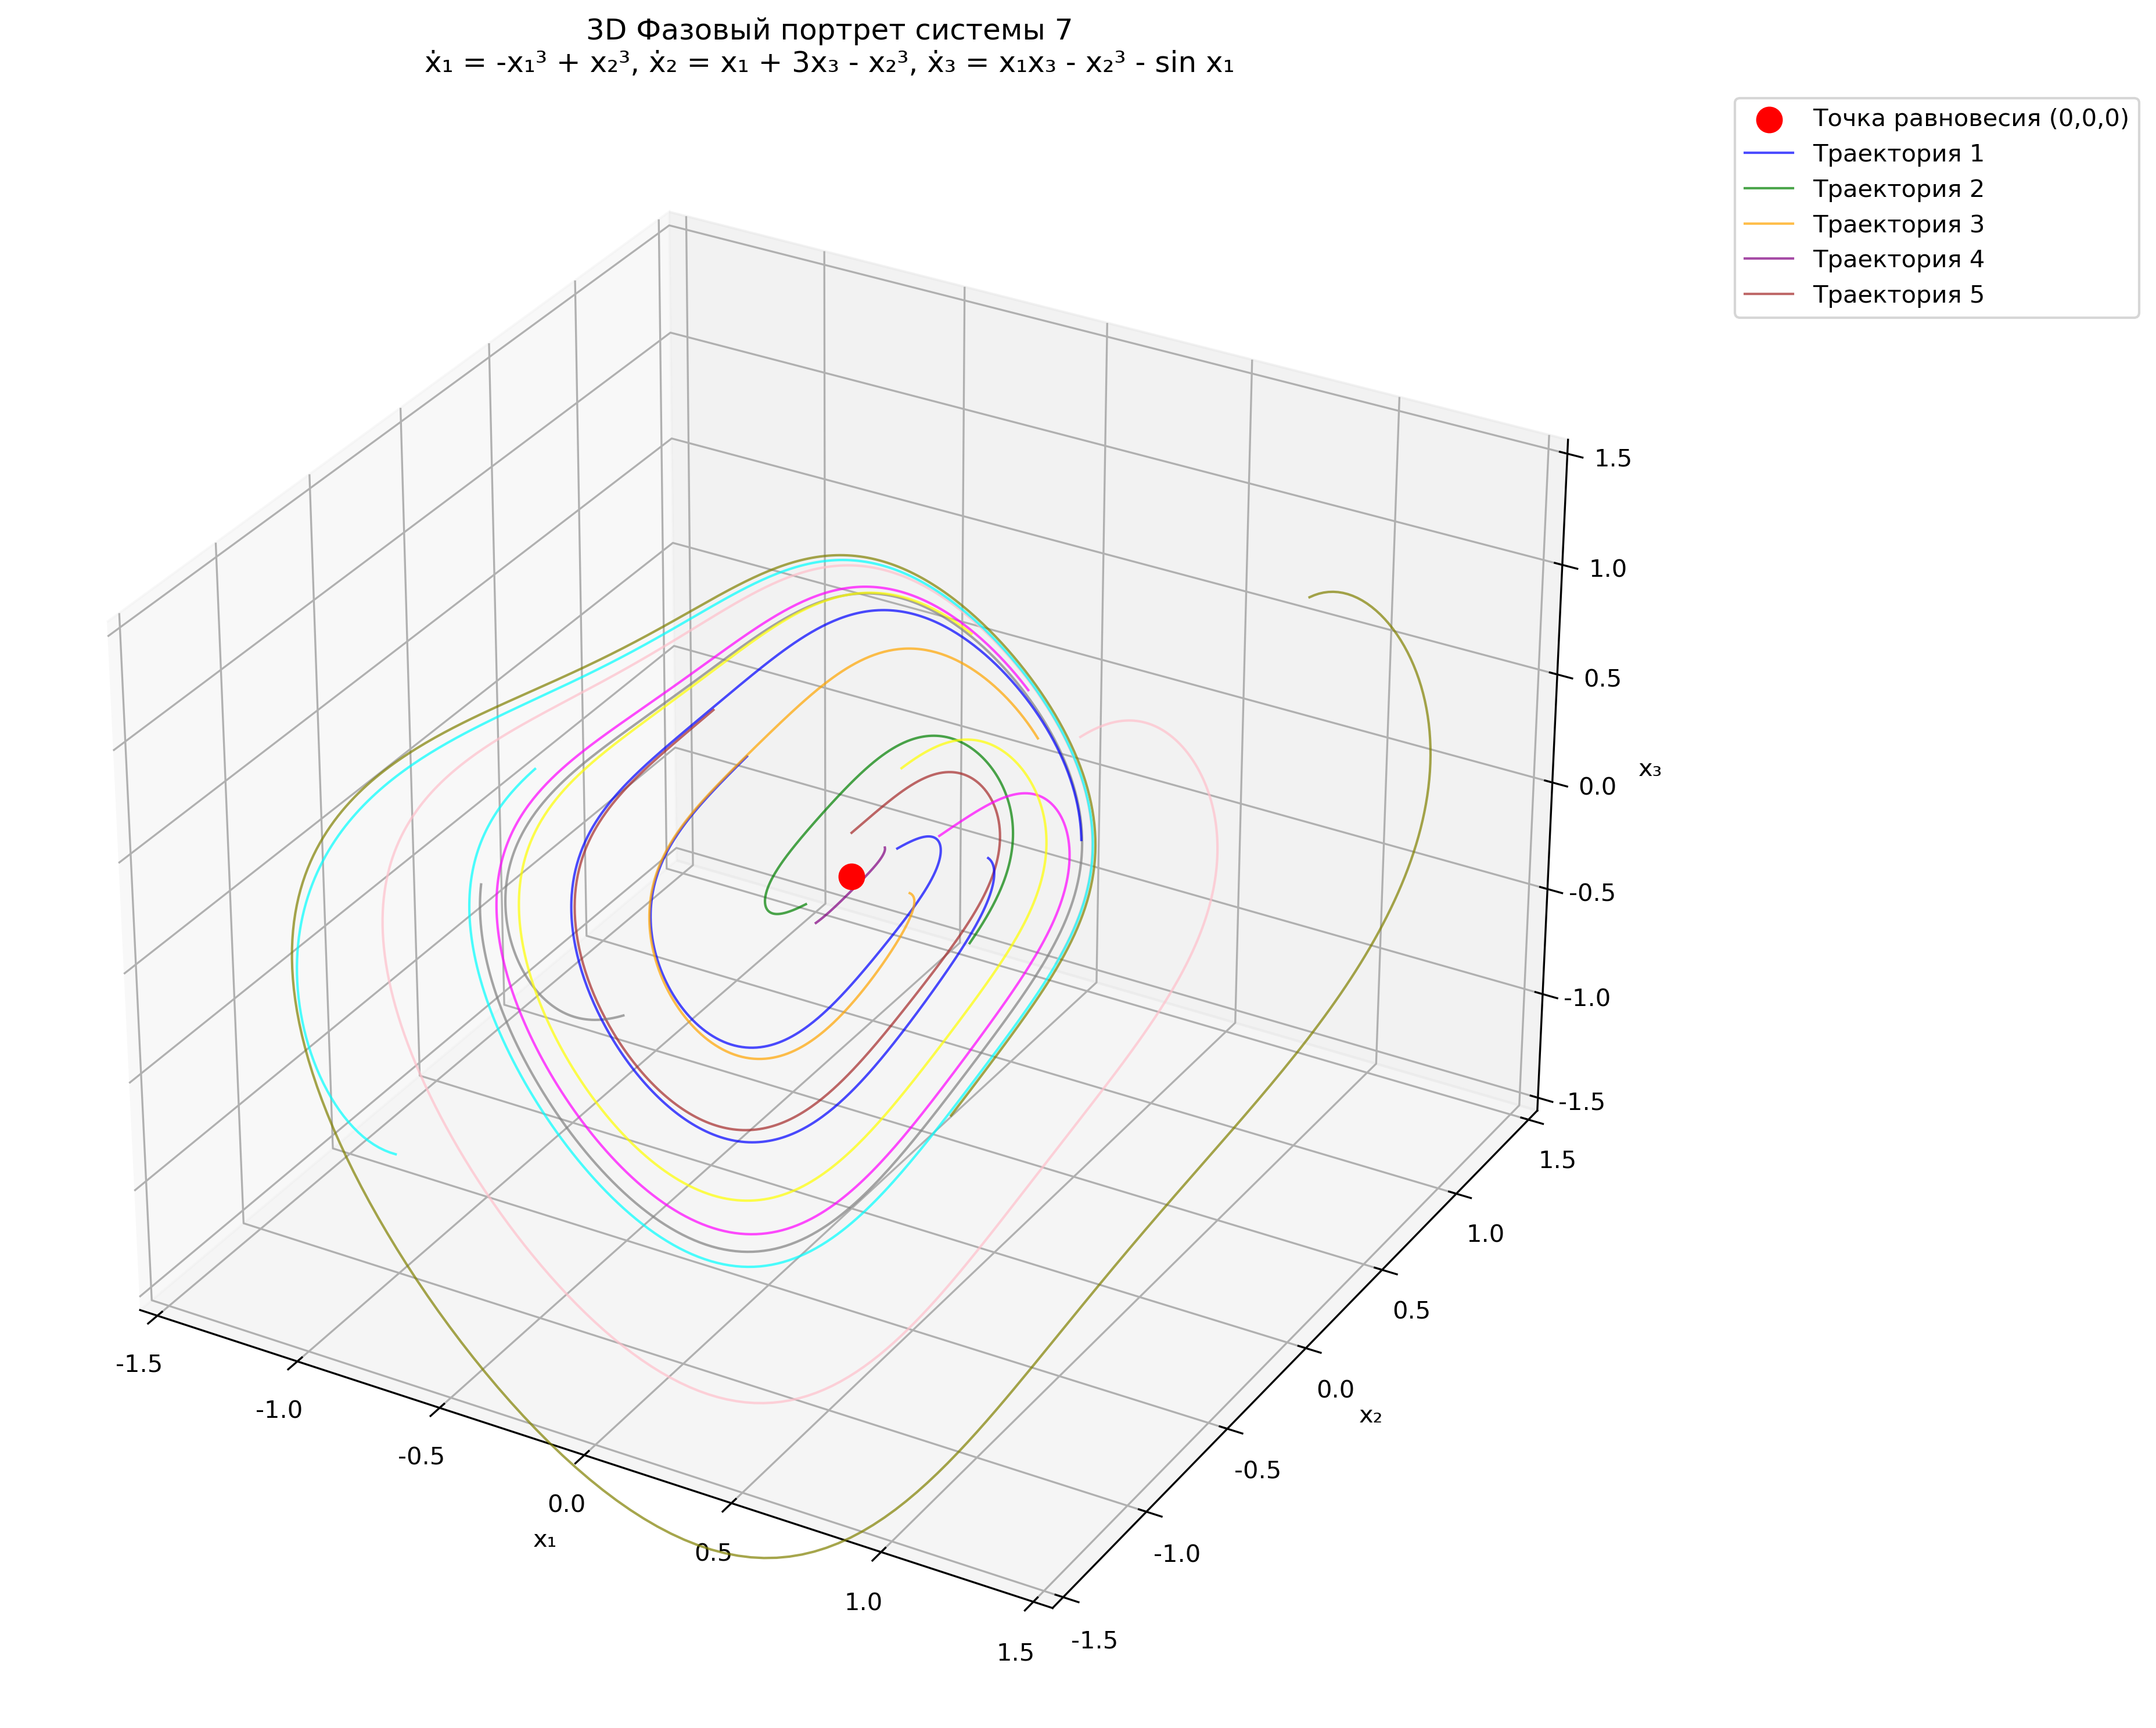
\includegraphics[width=\textwidth]{3d_systems/system7_3d_phase_portrait.png}
\caption{3D фазовый портрет системы 7}
\label{fig:system7_3d}
\end{subfigure}
\hfill
\begin{subfigure}[b]{0.49\textwidth}
\centering
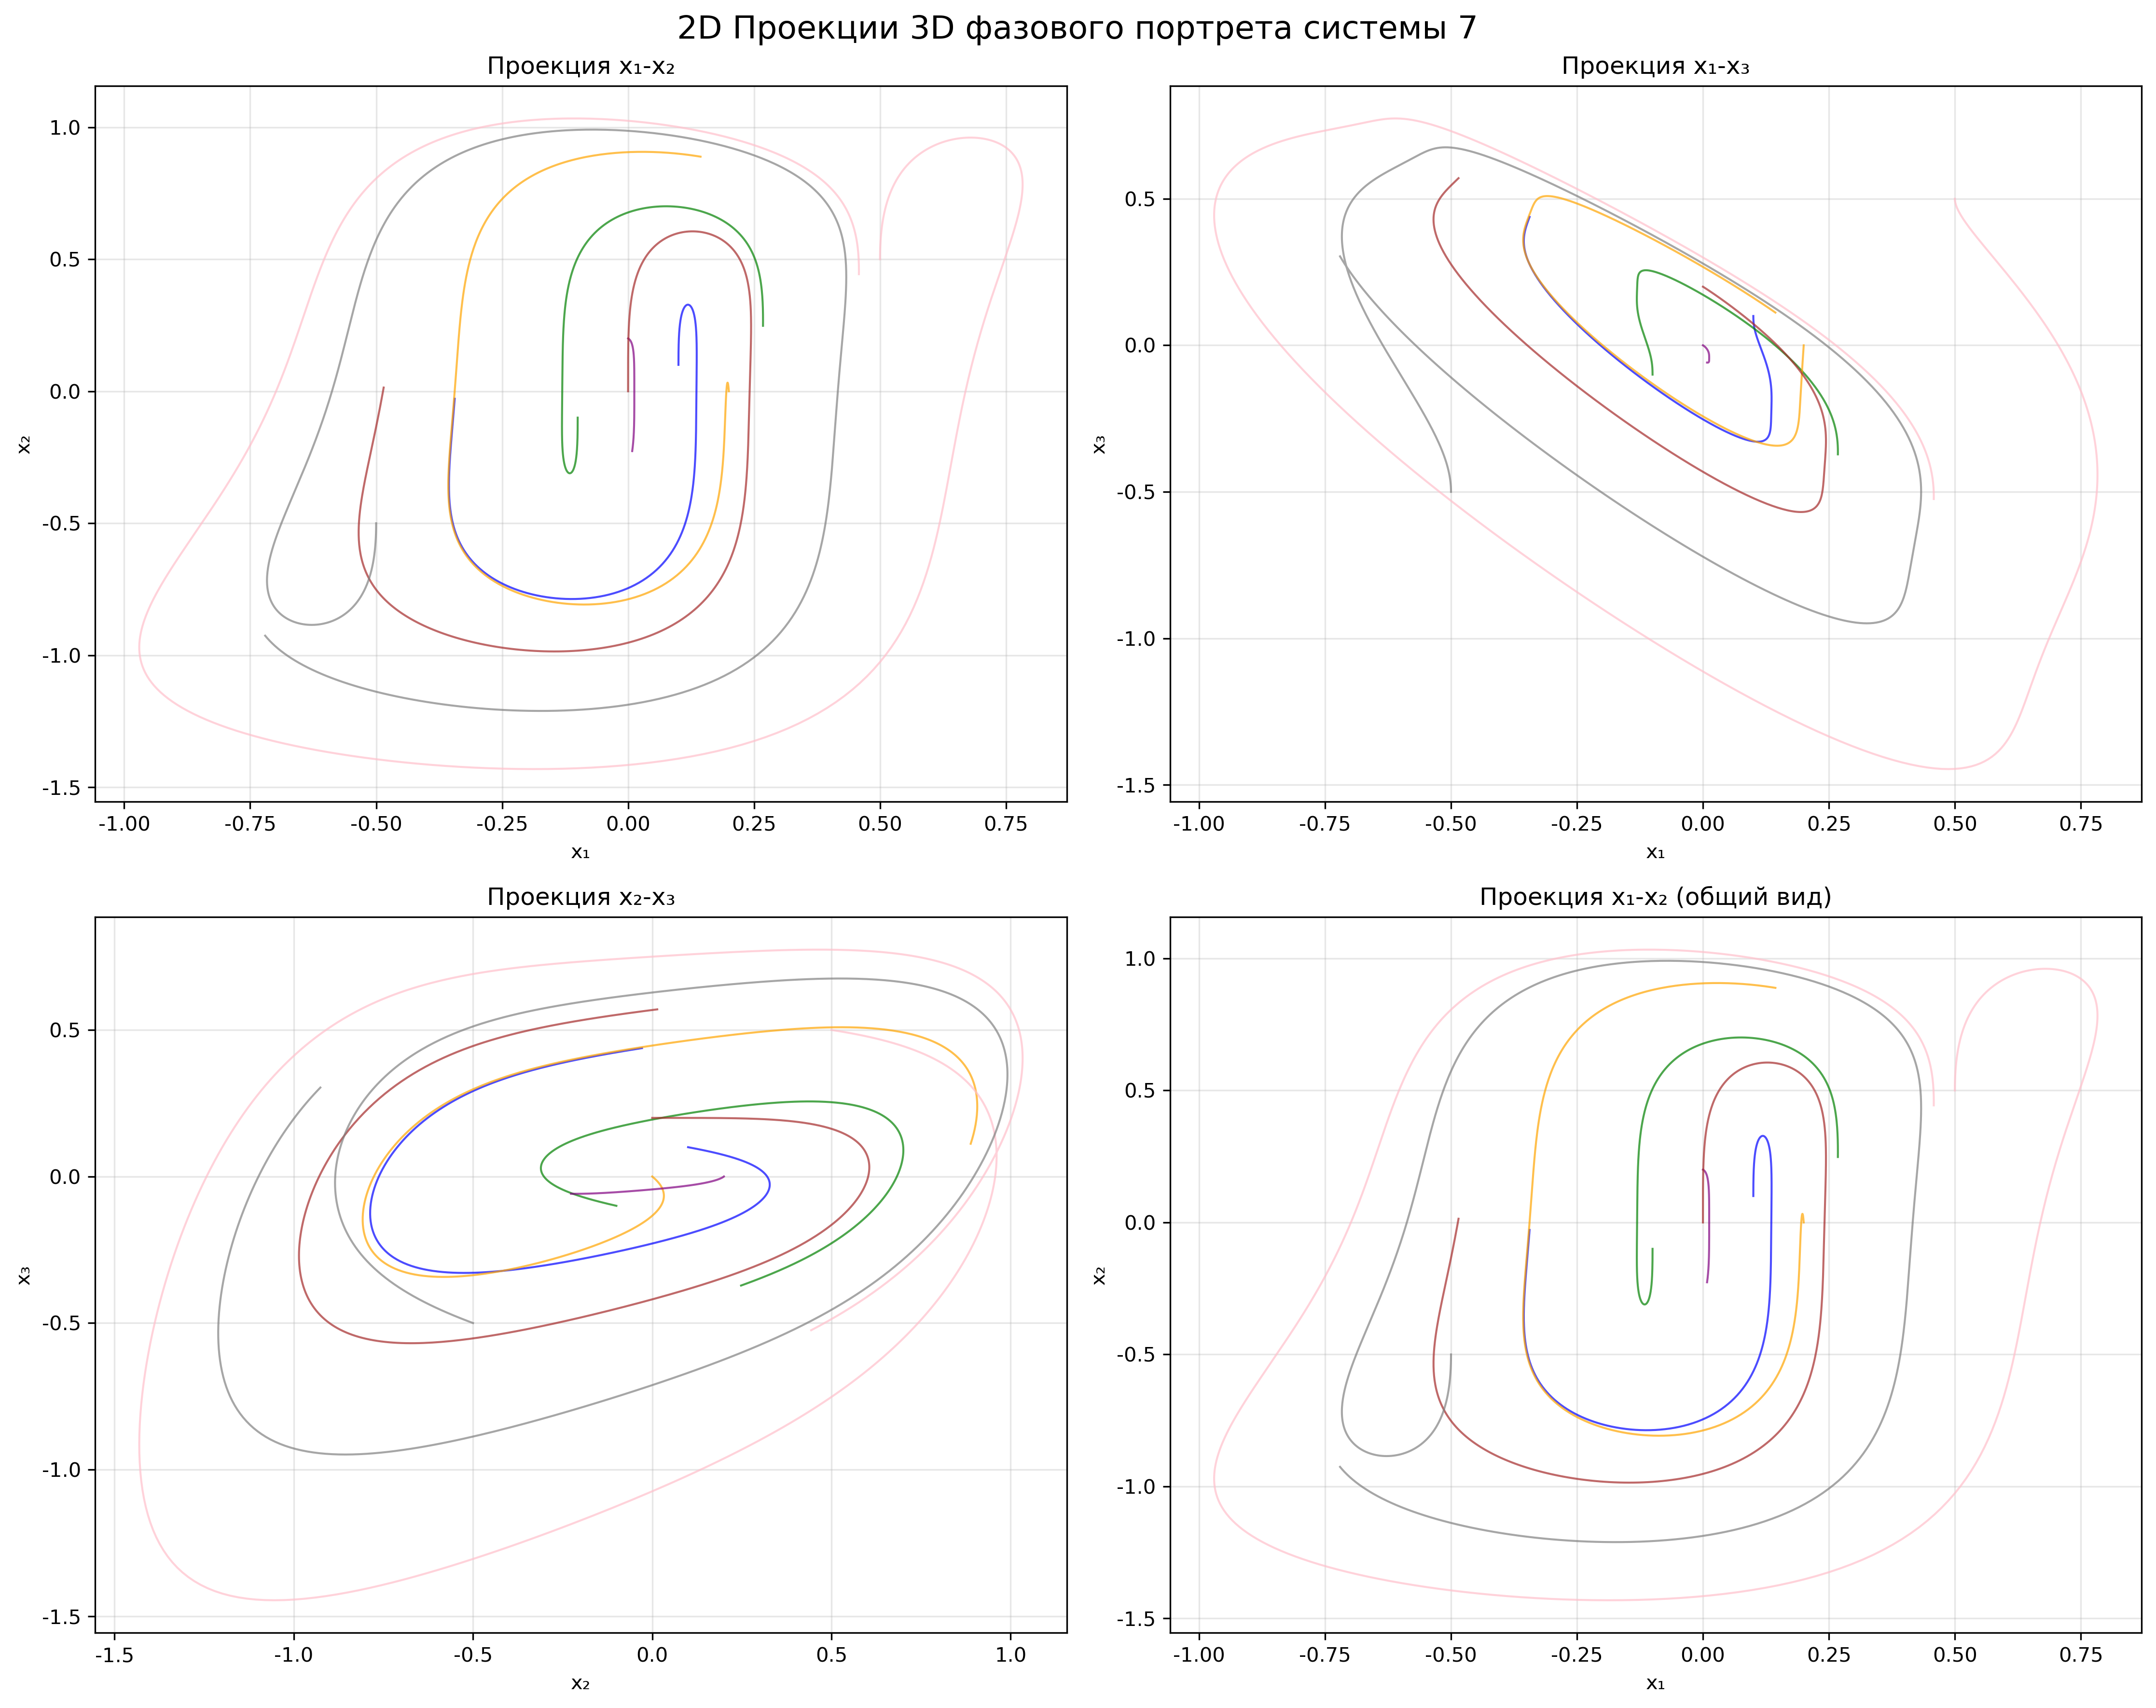
\includegraphics[width=\textwidth]{3d_systems/system7_2d_projections.png}
\caption{2D проекции фазового портрета системы 7}
\label{fig:system7_2d}
\end{subfigure}
\caption{Фазовые портреты системы 7}
\end{figure}

\subsection*{Анализ предельных циклов}

Для системы 4 проведен анализ предельных циклов с использованием перехода к полярным координатам.


\begin{figure}[H]
\centering
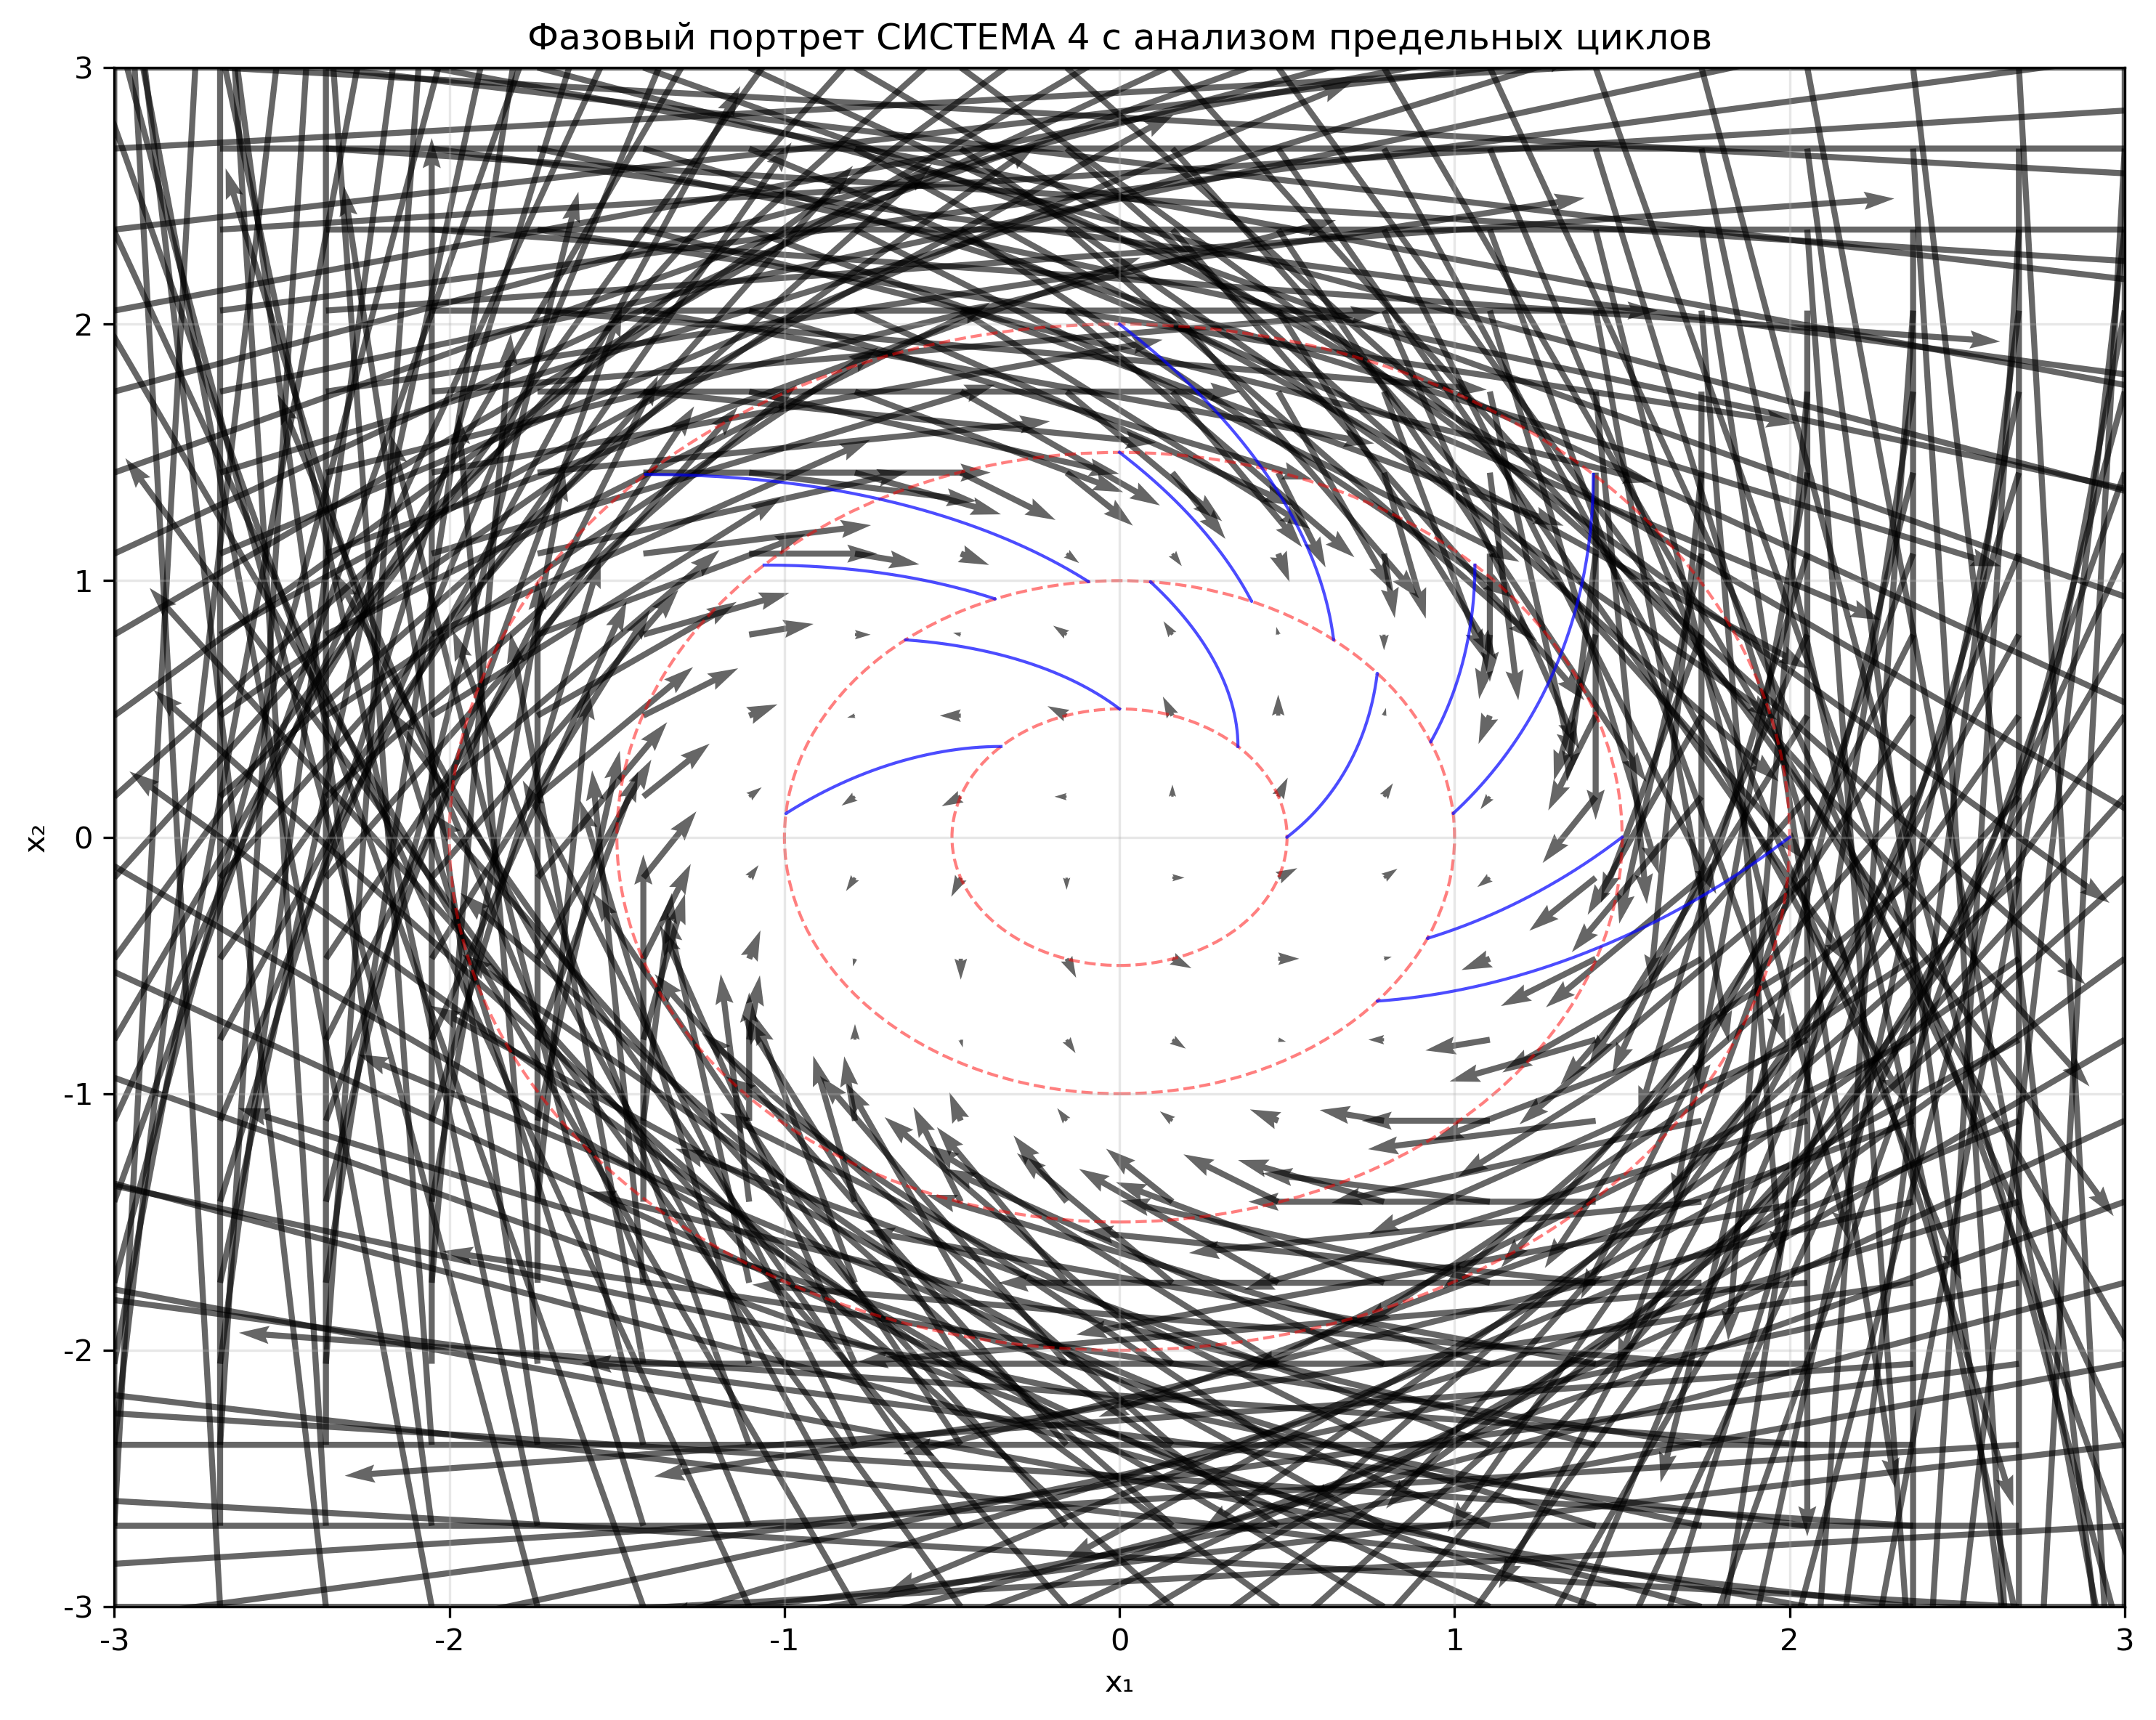
\includegraphics[width=0.8\textwidth]{limit_cycles/limit_cycles_система_4.png}
\caption{Фазовый портрет системы 4 с анализом предельных циклов}
\label{fig:limit_cycles_system4}
\end{figure}
                                  % Анализ систем
\section*{Синтез стабилизирующих регуляторов}

\subsection*{Управляемая система 1}

Рассмотрим систему:
\begin{align}
\dot{x}_1 &= -x_1 + 2x_1^3 + x_2 + \sin u_1 \\
\dot{x}_2 &= -x_1 - x_2 + 3\sin u_2
\end{align}

\subsubsection*{Выбор целевой точки и линеаризация по отклонениям}

Стабилизируем систему к точке вида $(1,y^*)$, где $y^*\in[-2,0]$ (это условие необходимо и достаточно для существования стационарных входов, см. ниже) и $y^*\neq -1$.
Из условий равновесия $f(1,y^*,u_{ss})=0$ получаем
\[
\sin u_{1,ss} = -(1+y^*),\qquad \sin u_{2,ss} = \frac{1+y^*}{3}.
\]
Для конкретики берём $y^*=-1.5$, тогда $u_{1,ss}=\arcsin(0.5)=\pi/6\approx0.524$, $u_{2,ss}=\arcsin(-0.5)= -\pi/6\approx-0.167$.
Линеаризуем систему по отклонениям $\tilde x = x - x^*$ и $v = u - u_{ss}$.

Матрицы Якоби в точке $(x^*,u_{ss})$ имеют вид:
\[
A = \left.\frac{\partial f}{\partial x}\right|_{(x^*,u_{ss})} =
\begin{pmatrix}
-1 + 6x_1^2 & 1 \\
-1 & -1
\end{pmatrix}_{x^*} =
\begin{pmatrix}
5 & 1 \\
-1 & -1
\end{pmatrix},\qquad
B = \left.\frac{\partial f}{\partial u}\right|_{(x^*,u_{ss})} =
\begin{pmatrix}
\cos u_{1,ss} & 0 \\
0 & 3\cos u_{2,ss}
\end{pmatrix} =
\begin{pmatrix}
\cos(\pi/6) & 0 \\
0 & 3\cos(-\pi/6)
\end{pmatrix} =
\begin{pmatrix}
0.8660 & 0 \\
0 & 2.9580
\end{pmatrix}.
\]

\subsubsection*{Синтез LQR}

Выберем $Q = 10I$, $R = I$ и решим алгебраическое уравнение Риккати
\[ A^T P + PA - PBR^{-1}B^T P + Q = 0,\quad K = R^{-1}B^T P. \]
Получаем матрицу обратной связи (численно)
\[
K = \begin{pmatrix}
11.7429 & 0.7194 \\
2.4573 & 3.0173
\end{pmatrix}.
\]
Спектр замкнутой линейной системы:
\[ \sigma(A-BK) = \{-5.9547,\;-9.1401\}. \]
Цель $(1,-1.5)$ локально экспоненциально устойчива; моделирование подтверждает сходимость траекторий к окрестности этой точки.

\subsection*{Управляемая система 2}

Рассмотрим систему:
\begin{align}
\dot{x}_1 &= x_2 + x_1 x_2 + u \\
\dot{x}_2 &= -x_2 + x_2^2 - x_1^3 + \sin u
\end{align}

\subsubsection*{Поиск точек равновесия}

При $u = 0$ система принимает вид:
\begin{align}
\dot{x}_1 &= x_2 + x_1 x_2 \\
\dot{x}_2 &= -x_2 + x_2^2 - x_1^3
\end{align}

Точки равновесия находятся из решения:
\begin{align}
x_2(1 + x_1) &= 0 \\
- x_2 + x_2^2 - x_1^3 &= 0
\end{align}

\textbf{Случай 1:} $x_2 = 0$. Из второго уравнения: $-x_1^3 = 0 \Rightarrow x_1 = 0$

\textbf{Случай 2:} $x_1 = -1$. Из второго уравнения: $-x_2 + x_2^2 - (-1)^3 = 0 \Rightarrow x_2^2 - x_2 + 1 = 0$.
Дискриминант: $D = 1 - 4 = -3 < 0$ --- нет действительных решений.

\textbf{Точка равновесия:} $(0, 0)$

\subsubsection*{Выбор точки равновесия и линеаризация}

Выберем точку равновесия $(x_1^*,x_2^*) = (0,0)$ и установим стационарный вход $u_{ss} = 0$.

Матрицы линейной модели:
\[
A = \begin{pmatrix} 0 & 1 \\ 0 & -1 \end{pmatrix},\qquad
B = \begin{pmatrix} 1 \\ 2 \end{pmatrix}.
\]
Для $Q=10I$, $R=1$ получаем
\[
K = \begin{pmatrix} 3.1623 & 2.1014 \end{pmatrix},\qquad
\sigma(A-BK) = \{-1.3529,\;-7.0121\}.
\]

\subsection*{Численное моделирование}

Результаты численного моделирования показывают эффективность синтезированных LQR регуляторов: для системы 1 траектории сходятся к точке $(1,-1.5)$, для системы 2 --- к $(0,0)$.

\begin{figure}[H]
\centering
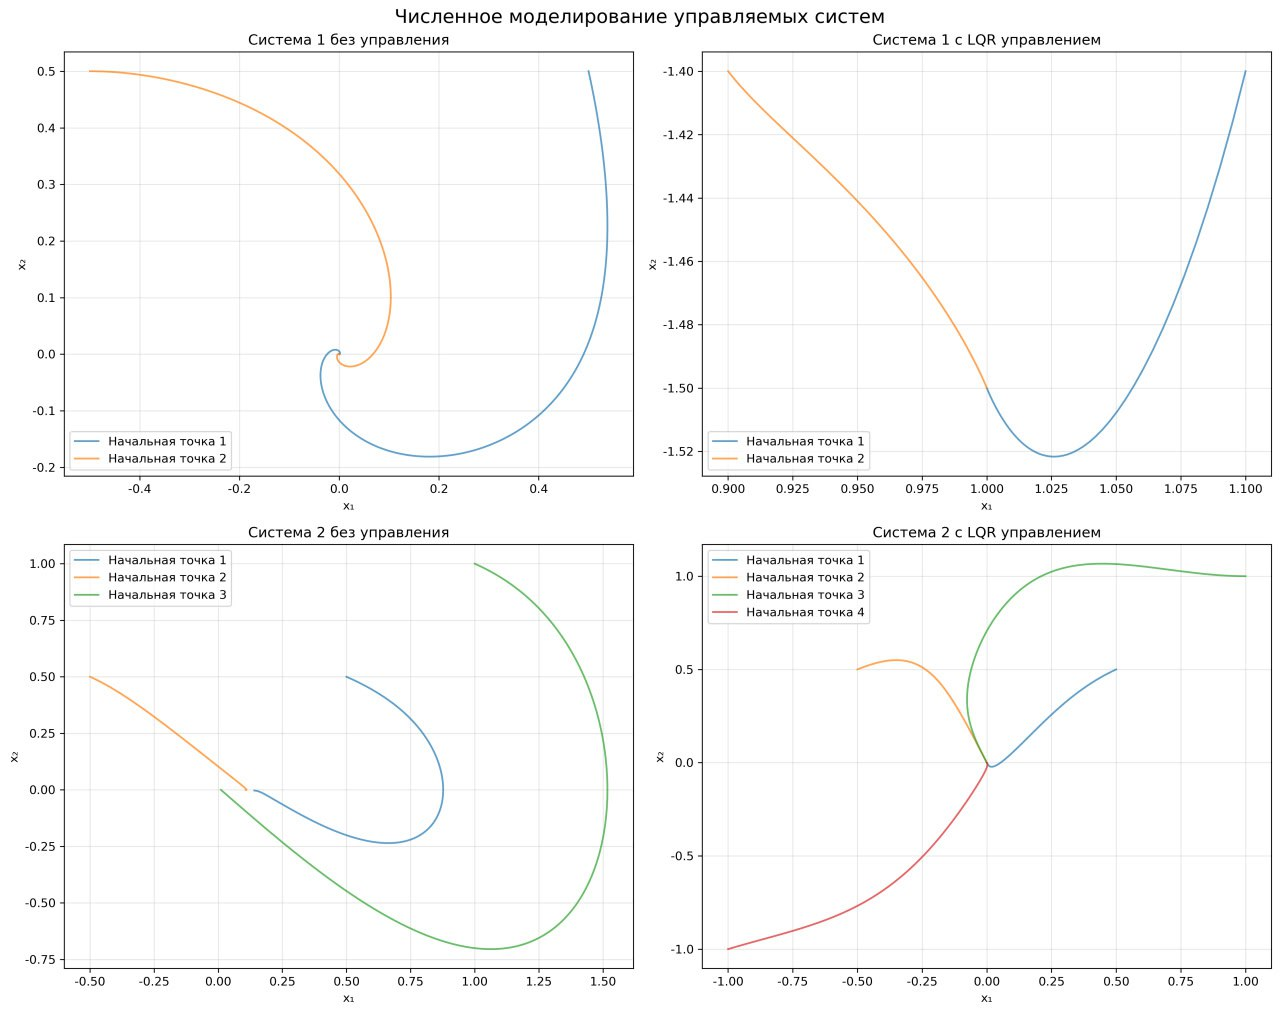
\includegraphics[width=0.8\textwidth]{controlled_systems/controller_simulation.png}
\caption{Результаты численного моделирования управляемых систем}
\label{fig:controller_sim}
\end{figure}
                        % Управляемые системы
\section*{Выводы}

В данной лабораторной работе был проведен комплексный анализ семи нелинейных динамических систем. Работа включала в себя поиск точек равновесия, классификацию их типов, построение фазовых портретов и синтез стабилизирующих регуляторов.

\begin{itemize}
\item \textbf{Анализ точек равновесия:} Для всех семи систем найдены точки равновесия аналитическими и численными методами;
\item \textbf{Классификация точек равновесия:} С использованием метода линеаризации определены типы всех изолированных точек равновесия;
\item \textbf{Фазовые портреты:} Построены численные фазовые портреты;
\item \textbf{Анализ предельных циклов:} Для систем 4 проведен анализ предельных циклов с использованием полярных координат;
\item \textbf{Синтез регуляторов:} Для двух управляемых систем синтезированы LQR регуляторы и проведено численное моделирование их работы.
\end{itemize}

Таким образом, методы анализа нелинейных систем, рассмотренные в работе, позволяют эффективно исследовать динамические свойства сложных систем и синтезировать стабилизирующие регуляторы.
                                % Заключение

\printbibliography[title=Список использованных источников] % Автособираемый список литературы

\end{document}
